%% Beispiel-Präsentation mit LaTeX Beamer im KIT-Design
%% entsprechend den Gestaltungsrichtlinien vom 1. August 2020
%%
%% Siehe https://sdqweb.ipd.kit.edu/wiki/Dokumentvorlagen

\documentclass[navbaroff,en]{sdqbeamer} 

\usepackage{comment}
\usepackage{tikz}
\usepackage{listings}
% \usepackage[demo]{graphicx}
\usepackage{subfigure}
 
%% Titelbild
\titleimage{banner_2020_kit}

%% Gruppenlogo
\grouplogo{}

%% Gruppenname
\groupname{IPD - Programming Paradigms Group}

% Beginn der Präsentation

\title{Compiler Presentation - Group 3}
\subtitle{Compiler Lab WS21/22}
\author[Nikolai, Pascal, Lars, Niklas]{Nikolai Maas, Pascal Mehnert, Lars König, Niklas Betten}

\date[10.\,2.\,2022]{10. February 2022}

\lstset{
    language=Java,
    basicstyle=\small\ttfamily,
    tabsize=4,
    columns=fixed,
    showstringspaces=false,
    showtabs=false,
    keepspaces,
    commentstyle=\color{red},
    keywordstyle=\color{blue}
}

\begin{document}

%Titelseite
\KITtitleframe

\begin{frame}
	\frametitle{Compiler Overview}

	\centering 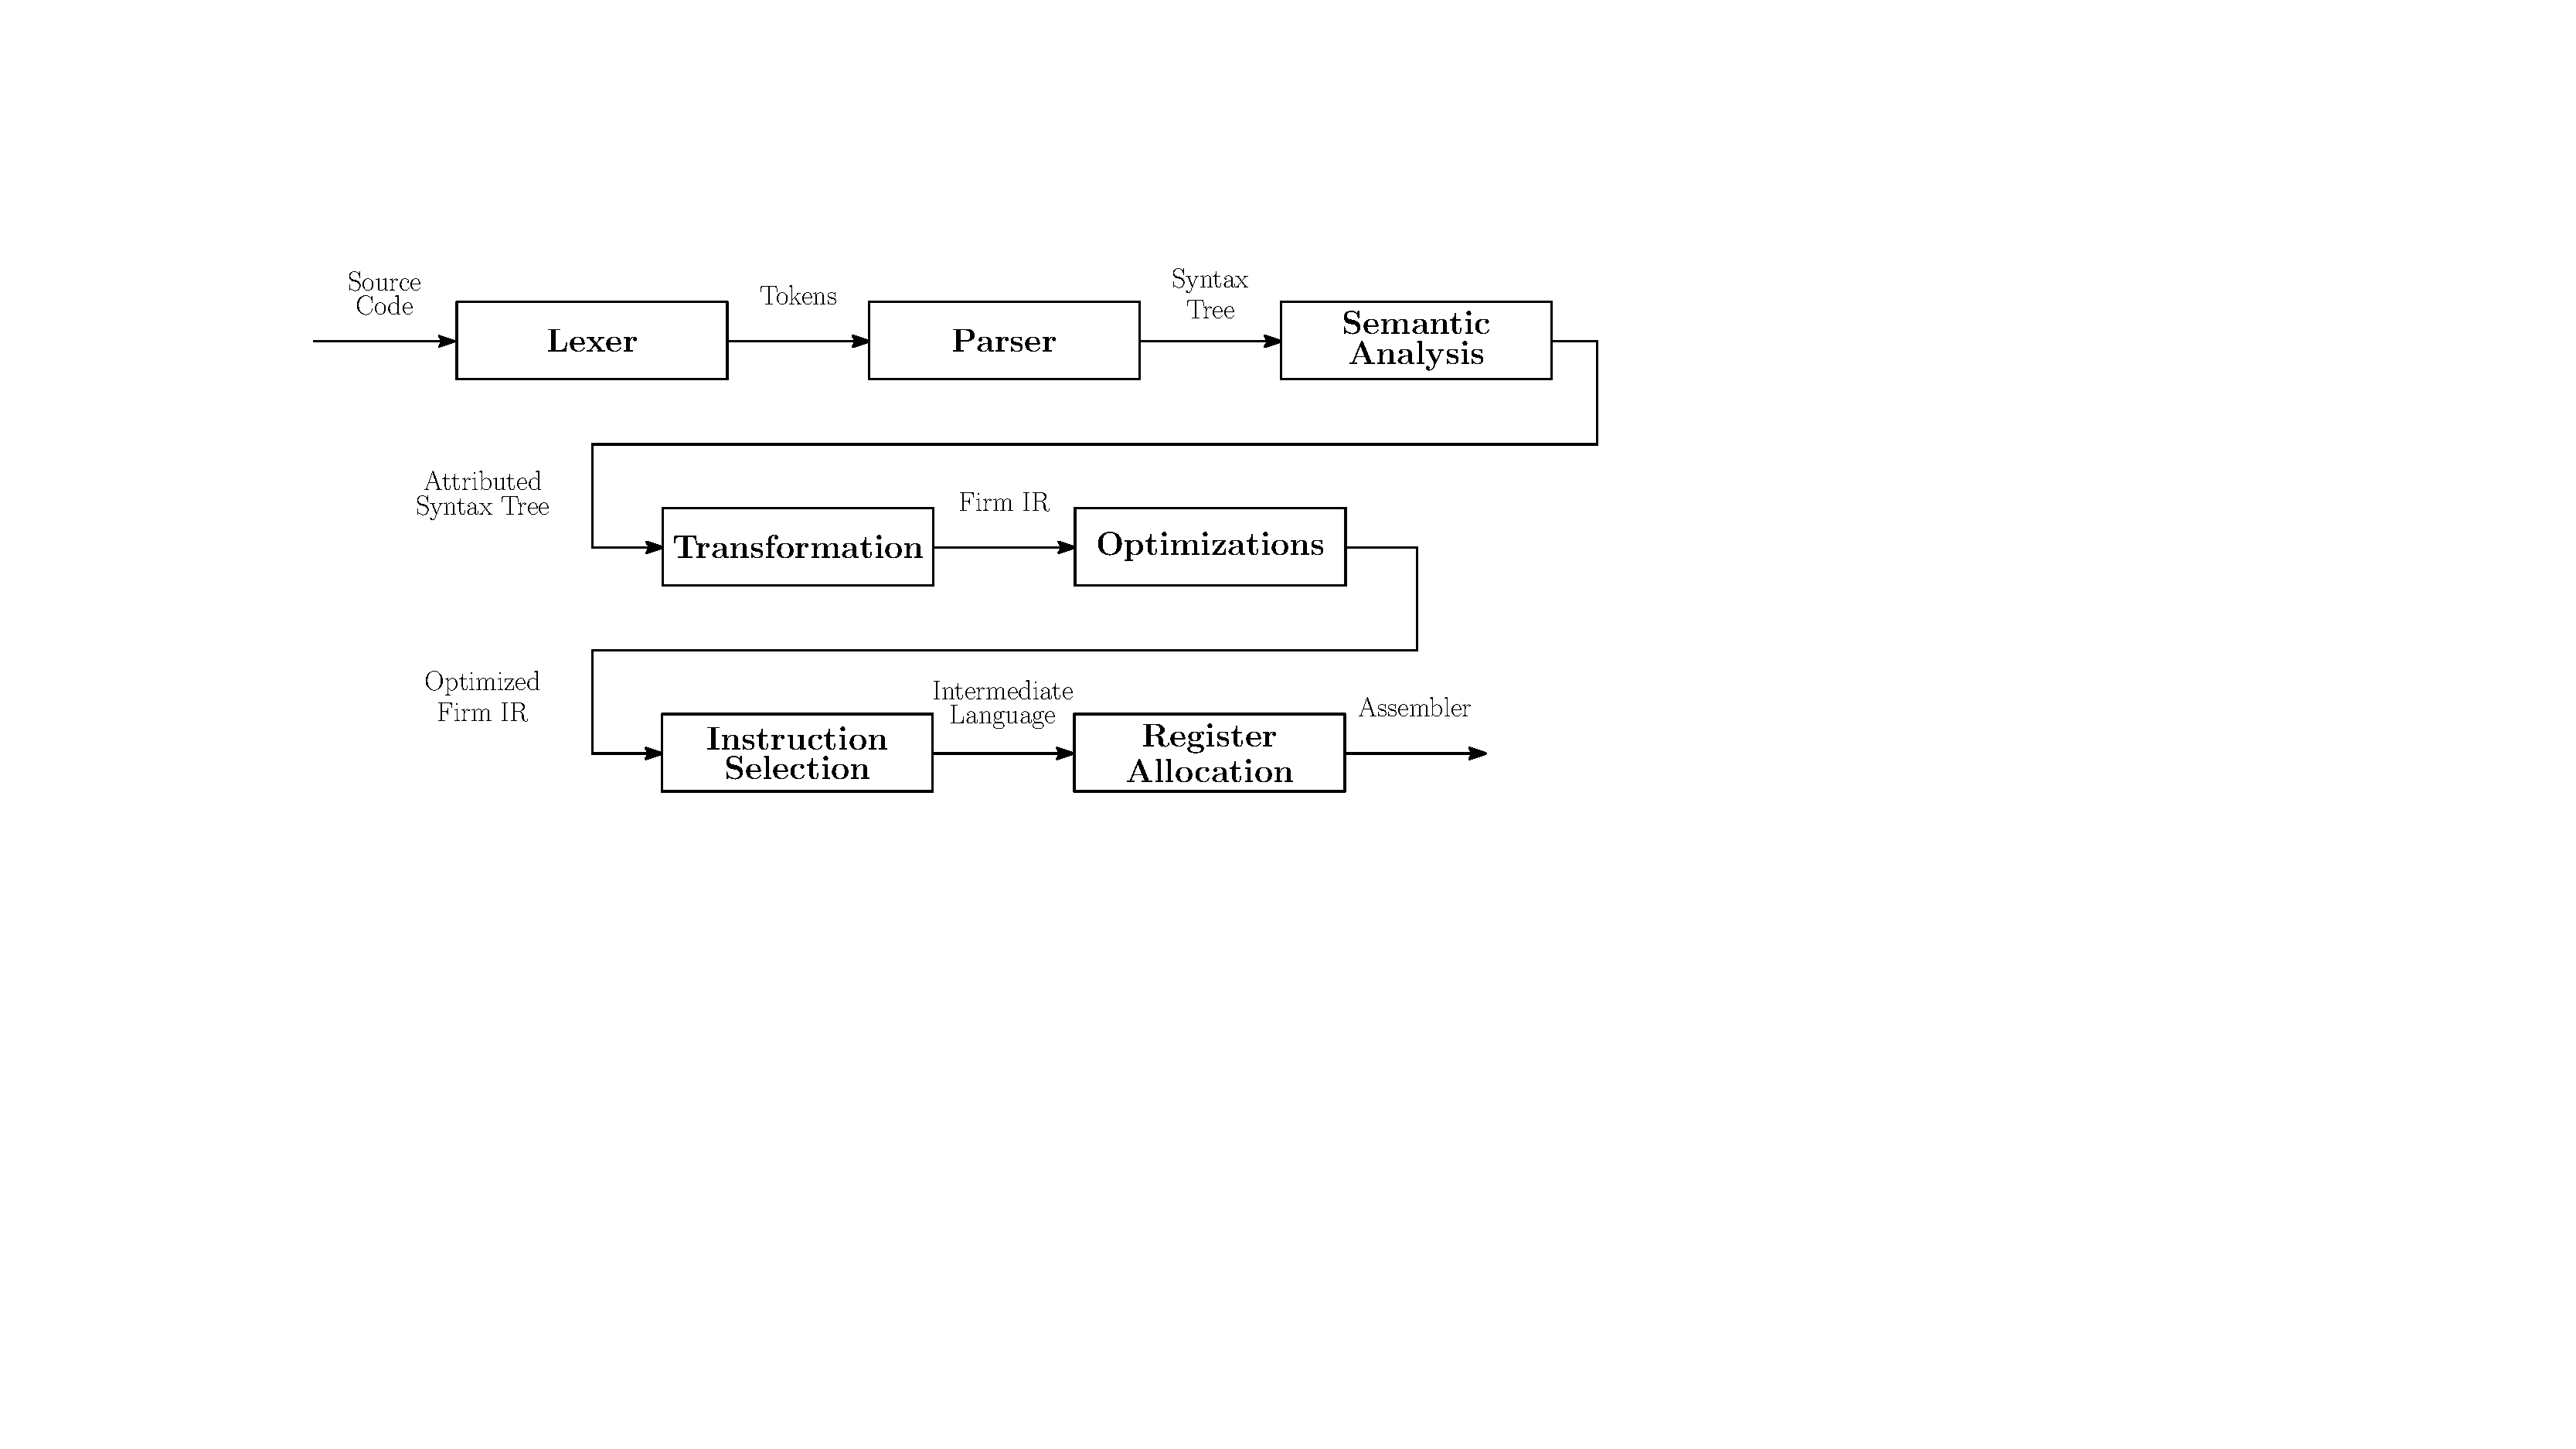
\includegraphics[scale=0.5]{images/phases.ipe.pdf}

\end{frame}


\section{Front End}

\begin{frame}
	\frametitle{Parser}

	\begin{itemize}
		\item \textbf{Input:} Tokens generated by Lexer
		\item Recursive descent pull parser
		\item Based on SLL(3) grammar
		\item Precedence climber for expressions
		\item No anchors $\,\longrightarrow\,$ No error recovery

		\vspace{1em}

		\item \textbf{Output:} Abstract Syntax Tree
		\item Major node types realized with inheritance
		\item Enums used to distinguish node sub-types
	\end{itemize}

\end{frame}

\begin{frame}
	\frametitle{Semantic Analysis}

	\begin{contentblock}{Namespace Gathering}
		\begin{itemize}
			\item Collect class, field, and method declarations
			\item Ensure existence of unique \texttt{main}-method
		\end{itemize}
	\end{contentblock}


	\begin{contentblock}{Name and Type Analysis}
		\begin{itemize}
			\item Find and link variable declarations
			\item Calculate expression result types
			\item Resolve function call references
		\end{itemize}
	\end{contentblock}


	\begin{contentblock}{Semantic Checks}
		\begin{itemize}
			\item Ensure existence of \texttt{return} statement on every path
			\item Ensure \texttt{args} and \texttt{String} are never used
			\item \dots and other miscellaneous checks
		\end{itemize}
	\end{contentblock}

\end{frame}

\begin{frame}
	\frametitle{Transformation}

	\begin{itemize}
		\item \textbf{Input:} Attributed AST
		\item Generate and cache Firm types
		\item Implemented using visitors on the AST

		\vspace{1em}

		\item Special handling for \textit{Div} and \textit{Mod}
		\begin{itemize}
			\item 32-bit division with explicit overflow checks
			\item \textit{(64-bit division several times slower)}
		\end{itemize}

		\vspace{1em}

		\item \textbf{Output:} Single Firm graph for each function
	\end{itemize}

\end{frame}


\section{Middle End}


\begin{frame}
	\frametitle{Optimizations -- Overview}

	\begin{columns}
		\begin{column}{0.48\textwidth}
			\begin{itemize}
				\item Constant Propagation
				\item Arithmetic Identities
				\item Trivial Jumps \& Linear Blocks
				\item Arithmetic Strength Reduction
				\item Pure Functions
				\item Inliner
				\item Loop Invariant Code Motion
				\item Loop Unrolling
				\item Common Subexpression Elimination

				\vspace{1em}

				\item Unused Arguments
			\end{itemize}
		\end{column}
		\begin{column}{0.48\textwidth}
			\lstinputlisting{firm/fibonacci/Fib.short.java}

			\begin{figure}
				\begin{minipage}{.3\textwidth}
					\centering
					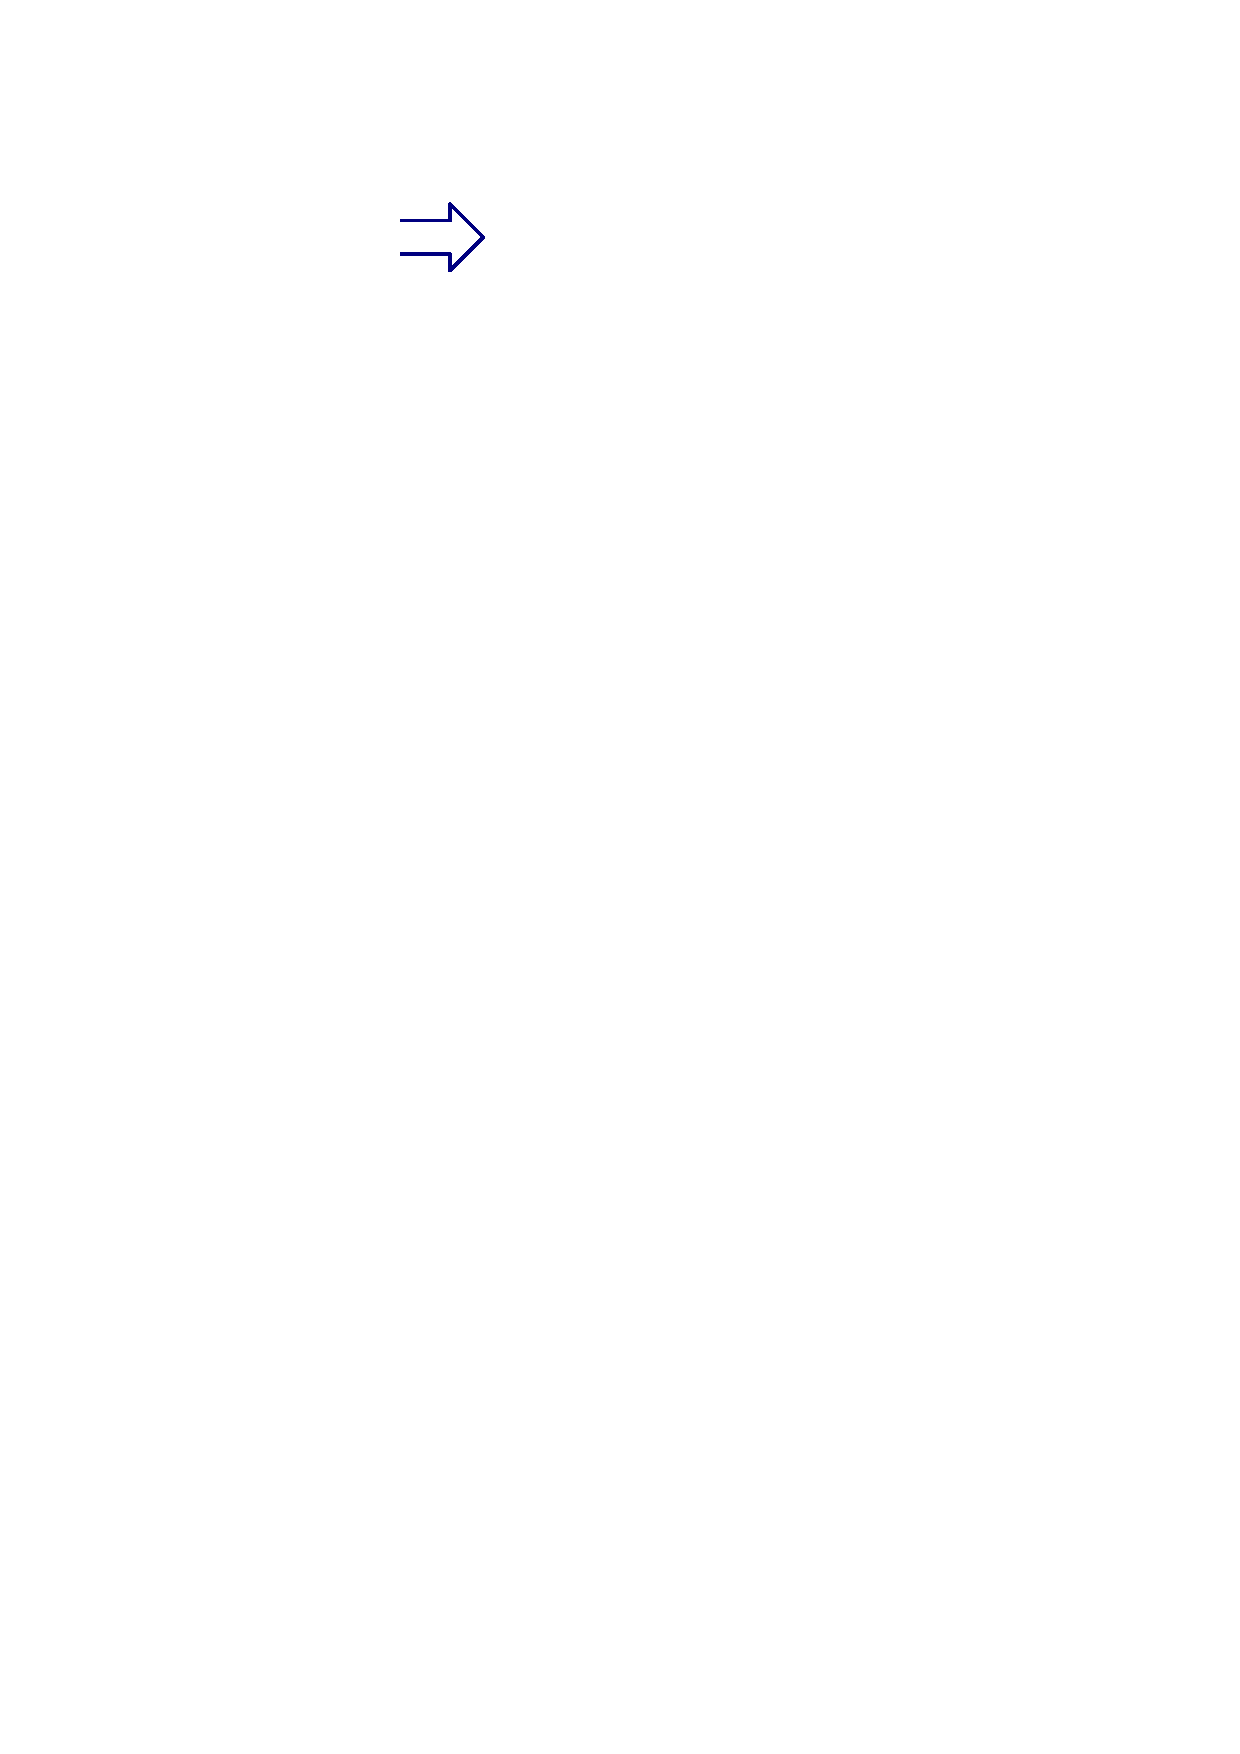
\includegraphics[scale=0.7]{images/arrow.ipe.pdf}
				\end{minipage}%
				\begin{minipage}{.6\textwidth}
					\centering
					\scalebox{0.115}{% Scale factor 0.12325581395348836
\definecolor{color20}{RGB}{255,153,153}
\definecolor{color21}{RGB}{255,255,153}
\definecolor{color22}{RGB}{153,153,255}
\definecolor{color23}{RGB}{255,153,255}
\definecolor{color24}{RGB}{100,100,255}
\definecolor{color25}{RGB}{0,0,0}
% Bounding Box: 248.0, 172.0
\begin{tikzpicture}
	\node[fill=color20, draw, minimum width=8.751162790697673cm, minimum height=3.7400885071865346cm] (n22) at (16.94767441860465cm ,-8.117663128431452cm) {};
	% 1 node layouts
	\node[scale=4.482029598308667, transform shape] at (16.94767441860465cm ,-8.117663128431452cm) {Return  92};
	\node[fill=color21, draw, minimum width=18.11860465116279cm, minimum height=3.7400885071865346cm] (n23) at (25.20581395348837cm ,0.5526579368946164cm) {};
	% 1 node layouts
	\node[scale=4.482029598308667, transform shape] at (25.20581395348837cm ,0.5526579368946164cm) {Const 0xFF80C38 Is 945};
	\node[fill=color22, draw, minimum width=9.983720930232558cm, minimum height=3.7400885071865346cm] (n24) at (8.68953488372093cm ,0.5526579368946164cm) {};
	% 1 node layouts
	\node[scale=4.482029598308667, transform shape] at (8.68953488372093cm ,0.5526579368946164cm) {Proj M M 70};
	\node[fill=color23, draw, minimum width=7.51860465116279cm, minimum height=3.7400885071865346cm] (n25) at (8.68953488372093cm ,9.222979002220685cm) {};
	% 1 node layouts
	\node[scale=4.482029598308667, transform shape] at (8.68953488372093cm ,9.222979002220685cm) {Start  67};
	\draw[color=color24, -latex] (14.759883720930231cm ,-6.247618874838185cm) -- (14.759883720930231cm ,-3.782502595768418cm) -- (8.68953488372093cm ,-3.782502595768418cm) -- (8.68953488372093cm ,-1.3173863166986508cm);
	\node[] at (15.684302325581394cm ,-4.4527060841405115cm) {
		\scalebox{4.482029598308667}{0}
	};
	\draw[color=color25, -latex] (19.135465116279068cm ,-6.247618874838185cm) -- (19.135465116279068cm ,-3.782502595768418cm) -- (25.20581395348837cm ,-3.782502595768418cm) -- (25.20581395348837cm ,-1.3173863166986508cm);
	\node[] at (20.05988372093023cm ,-4.4527060841405115cm) {
		\scalebox{4.482029598308667}{1}
	};
	\draw[color=color24, -latex] (8.68953488372093cm ,2.422702190487884cm) -- (8.68953488372093cm ,7.352934748627418cm);
	\node[] at (9.613953488372092cm ,4.887818469557651cm) {
		\scalebox{4.482029598308667}{0}
	};
\end{tikzpicture}
}
				\end{minipage}
			\end{figure}
		\end{column}
	\end{columns}

\end{frame}


\begin{frame}
    \frametitle{Optimizations -- Fixed Point Iterations}

	\begin{contentblock}{Call Graph}
		\begin{itemize}
			\item Used to walk functions in bottom-up order
			\item Passed to optimizations ($\rightarrow$ Inliner)
			\item Detect and prune dead functions
		\end{itemize}
	\end{contentblock}

	\begin{contentblock}{Local Optimizations}
		\begin{itemize}
			\item Applied to a single function
			\item Run all optimizations until FP is reached
		\end{itemize}
	\end{contentblock}

	\begin{contentblock}{Global Optimizations}
		\begin{itemize}
			\item Run on the entire program
			\item Return the set of changed functions
		\end{itemize}
	\end{contentblock}

\end{frame}

\begin{frame}
    \frametitle{Loop Unrolling}

	\begin{columns}
		\begin{column}{0.48\textwidth}
			\begin{itemize}
				\item[1.] Find closed natural loops
				\item[2.] Find loop variables
				\item[3.] Determine loop boundaries
				\item[4.] Calculate number of iterations
			\end{itemize}
		\end{column}
		\begin{column}{0.25\textwidth}
			\centering
			\scalebox{0.2}{%
				% Scale factor 0.0398936170212766
\definecolor{color39}{RGB}{222,239,234}
\definecolor{color40}{RGB}{255,153,153}
\definecolor{color41}{RGB}{0,150,60}
\definecolor{color42}{RGB}{255,255,255}
\definecolor{color43}{RGB}{255,255,153}
\definecolor{color44}{RGB}{153,255,153}
\definecolor{color45}{RGB}{255,0,0}
\definecolor{color46}{RGB}{0,0,0}
% Bounding Box: 376.0, 771.0
\begin{tikzpicture}
	\node[fill=color39, draw, minimum width=3.390957446808511cm, minimum height=3.444579028068705cm] (n103) at (11.141954787234042cm ,29.035689209369906cm) {};
	% 1 node layouts
	\node[scale=1.4506769825918764, transform shape] at (11.141954787234042cm ,30.24350976690333cm) {Start Block  64};
	\node[fill=color39, draw, minimum width=9.73404255319149cm, minimum height=8.64447720507358cm] (n104) at (5.285904255319149cm ,5.1299680801148115cm) {};
	% 1 node layouts
	\node[scale=1.4506769825918764, transform shape] at (5.285904255319149cm ,8.937737726150676cm) {Block  76};
	\node[fill=color39, draw, minimum width=10.605053191489365cm, minimum height=14.669703650981823cm] (n105) at (8.490691489361701cm ,18.382803188993577cm) {};
	% 1 node layouts
	\node[scale=1.4506769825918764, transform shape] at (8.490691489361701cm ,25.20318605798356cm) {Block  74};
	\node[fill=color39, draw, minimum width=4.029255319148937cm, minimum height=5.838196049345301cm] (n106) at (12.965425531914894cm ,5.1299680801148115cm) {};
	% 1 node layouts
	\node[scale=1.4506769825918764, transform shape] at (12.965425531914894cm ,7.534597148286536cm) {Block  77};
	\node[fill=color40, draw, minimum width=2.8324468085106385cm, minimum height=1.2105364748772156cm] (n107) at (12.965425531914894cm ,3.4145425481999174cm) {};
	% 1 node layouts
	\node[scale=1.4506769825918764, transform shape] at (12.965425531914894cm ,3.4145425481999174cm) {Return  87};
	\node[fill=color41, draw, minimum width=0.7978723404255319cm, minimum height=0.7978723404255319cm] (n108) at (12.965425531914894cm ,6.014491636702355cm) {};
	\node[fill=color40, draw, minimum width=3.7101063829787235cm, minimum height=1.2105364748772156cm] (n109) at (11.339760638297873cm ,12.251623856260423cm) {};
	% 1 node layouts
	\node[scale=1.4506769825918764, transform shape] at (11.339760638297873cm ,12.251623856260423cm) {Proj X false 83};
	\node[fill=color40, draw, minimum width=3.550531914893617cm, minimum height=1.2105364748772156cm] (n110) at (6.911569148936169cm ,12.251623856260423cm) {};
	% 1 node layouts
	\node[scale=1.4506769825918764, transform shape] at (6.911569148936169cm ,12.251623856260423cm) {Proj X true 82};
	\node[fill=color40, draw, minimum width=2.513297872340426cm, minimum height=1.2105364748772156cm] (n111) at (9.215425531914892cm ,15.057905011988701cm) {};
	% 1 node layouts
	\node[scale=1.4506769825918764, transform shape] at (9.215425531914892cm ,15.057905011988701cm) {Cond  81};
	\node[fill=color42, draw, minimum width=3.670212765957447cm, minimum height=1.2105364748772156cm] (n112) at (9.215425531914892cm ,17.86418616771698cm) {};
	% 1 node layouts
	\node[scale=1.4506769825918764, transform shape] at (9.215425531914892cm ,17.86418616771698cm) {Cmp b less 80};
	\node[fill=color43, draw, minimum width=3.9494680851063833cm, minimum height=1.2105364748772156cm] (n113) at (10.132978723404253cm ,20.670467323445262cm) {};
	% 1 node layouts
	\node[scale=1.4506769825918764, transform shape] at (10.132978723404253cm ,20.670467323445262cm) {Const 0x4 Is 79};
	\node[fill=color44, draw, minimum width=2.4335106382978724cm, minimum height=1.2105364748772156cm] (n114) at (6.053856382978722cm ,20.670467323445262cm) {};
	% 1 node layouts
	\node[scale=1.4506769825918764, transform shape] at (6.053856382978722cm ,20.670467323445262cm) {Phi Is 78};
	\node[fill=color43, draw, minimum width=3.9494680851063833cm, minimum height=1.2105364748772156cm] (n115) at (7.3570478723404245cm ,23.47674847917354cm) {};
	% 1 node layouts
	\node[scale=1.4506769825918764, transform shape] at (7.3570478723404245cm ,23.47674847917354cm) {Const 0x0 Is 72};
	\node[fill=color41, draw, minimum width=0.7978723404255319cm, minimum height=0.7978723404255319cm] (n116) at (4.567819148936168cm ,17.86418616771698cm) {};
	\node[fill=color41, draw, minimum width=0.7978723404255319cm, minimum height=0.7978723404255319cm] (n117) at (4.185505319148934cm ,23.47674847917354cm) {};
	\node[fill=color41, draw, minimum width=0.7978723404255319cm, minimum height=0.7978723404255319cm] (n118) at (6.163563829787232cm ,17.86418616771698cm) {};
	\node[fill=color40, draw, minimum width=2.1941489361702127cm, minimum height=1.2105364748772156cm] (n119) at (2.1143617021276597cm ,7.211300147340653cm) {};
	% 1 node layouts
	\node[scale=1.4506769825918764, transform shape] at (2.1143617021276597cm ,7.211300147340653cm) {Jmp  86};
	\node[fill=color42, draw, minimum width=2.6329787234042556cm, minimum height=1.2105364748772156cm] (n120) at (7.569813829787234cm ,4.405018991612374cm) {};
	% 1 node layouts
	\node[scale=1.4506769825918764, transform shape] at (7.569813829787234cm ,4.405018991612374cm) {Add Is 85};
	\node[fill=color43, draw, minimum width=3.9494680851063833cm, minimum height=1.2105364748772156cm] (n121) at (5.98404255319149cm ,7.211300147340653cm) {};
	% 1 node layouts
	\node[scale=1.4506769825918764, transform shape] at (5.98404255319149cm ,7.211300147340653cm) {Const 0x1 Is 84};
	\node[fill=color41, draw, minimum width=0.7978723404255319cm, minimum height=0.7978723404255319cm] (n122) at (9.15558510638298cm ,7.211300147340653cm) {};
	\node[fill=color41, draw, minimum width=0.7978723404255319cm, minimum height=0.7978723404255319cm] (n123) at (7.569813829787233cm ,1.8050699031099362cm) {};
	\node[fill=color40, draw, minimum width=2.1941489361702127cm, minimum height=1.2105364748772156cm] (n124) at (11.141954787234042cm ,28.51707218809331cm) {};
	% 1 node layouts
	\node[scale=1.4506769825918764, transform shape] at (11.141954787234042cm ,28.51707218809331cm) {Jmp  73};
	\draw[color=color45, -latex] (11.141954787234042cm ,25.71765501448449cm) -- (11.141954787234042cm ,27.9118039506547cm);
	\node[] at (11.441156914893616cm ,26.52737803915714cm) {
		\scalebox{1.4506769825918764}{0}
	};
	\draw[color=color45, -latex] (5.839428191489361cm ,25.71765501448449cm) -- (5.839428191489359cm ,26.51552735491002cm) -- (0.0cm ,26.51552735491002cm) -- (0.0cm ,0.009857137152489197cm) -- (2.1143617021276597cm ,0.009857137152489197cm) -- (2.1143617021276597cm ,6.606031909902045cm);
	\node[] at (6.138630319148934cm ,26.29860581235683cm) {
		\scalebox{1.4506769825918764}{1}
	};
	\draw[color=color45, -latex] (12.965425531914894cm ,8.049066104787462cm) -- (12.965425531914894cm ,10.250079023077133cm) -- (11.339760638297873cm ,10.250079023077133cm) -- (11.339760638297873cm ,11.646355618821815cm);
	\node[] at (13.264627659574469cm ,8.858789129460112cm) {
		\scalebox{1.4506769825918764}{0}
	};
	\draw[color=color45, -latex] (5.285904255319149cm ,9.452206682651601cm) -- (5.285904255319149cm ,10.250079023077133cm) -- (6.911569148936169cm ,10.250079023077133cm) -- (6.911569148936169cm ,11.646355618821815cm);
	\node[] at (5.585106382978724cm ,10.033157480523942cm) {
		\scalebox{1.4506769825918764}{0}
	};
	\draw[color=color46, -latex] (12.965425531914894cm ,4.0198107856385255cm) -- (12.965425531914894cm ,5.615555466489589cm);
	\node[] at (13.264627659574469cm ,4.817683126064058cm) {
		\scalebox{1.4506769825918764}{1}
	};
	\draw[color=color45, -latex] (11.339760638297873cm ,12.85689209369903cm) -- (11.339760638297873cm ,13.654764434124562cm) -- (9.843749999999998cm ,13.654764434124562cm) -- (9.843749999999998cm ,14.452636774550093cm);
	\node[] at (11.638962765957448cm ,13.43784289157137cm) {
		\scalebox{1.4506769825918764}{0}
	};
	\draw[color=color45, -latex] (6.911569148936169cm ,12.85689209369903cm) -- (6.911569148936169cm ,13.654764434124562cm) -- (8.587101063829785cm ,13.654764434124562cm) -- (8.587101063829785cm ,14.452636774550093cm);
	\node[] at (7.210771276595744cm ,13.43784289157137cm) {
		\scalebox{1.4506769825918764}{0}
	};
	\draw[color=color46, -latex] (9.215425531914892cm ,15.66317324942731cm) -- (9.215425531914892cm ,17.258917930278372cm);
	\node[] at (9.514627659574467cm ,16.46104558985284cm) {
		\scalebox{1.4506769825918764}{0}
	};
	\draw[color=color46, -latex] (8.29787234042553cm ,18.469454405155588cm) -- (8.29787234042553cm ,19.26732674558112cm) -- (6.86502659574468cm ,19.26732674558112cm) -- (6.86502659574468cm ,20.065199086006654cm);
	\node[] at (8.597074468085104cm ,19.05040520302793cm) {
		\scalebox{1.4506769825918764}{0}
	};
	\draw[color=color46, -latex] (10.132978723404253cm ,18.469454405155588cm) -- (10.132978723404253cm ,20.065199086006654cm);
	\node[] at (10.432180851063828cm ,19.26732674558112cm) {
		\scalebox{1.4506769825918764}{1}
	};
	\draw[color=color46, -latex] (6.662234042553191cm ,21.275735560883867cm) -- (6.662234042553191cm ,22.0736079013094cm) -- (7.3570478723404245cm ,22.0736079013094cm) -- (7.3570478723404245cm ,22.871480241734933cm);
	\node[] at (6.961436170212766cm ,21.856686358756207cm) {
		\scalebox{1.4506769825918764}{0}
	};
	\draw[color=color46, -latex] (5.445478723404254cm ,21.275735560883867cm) -- (5.445478723404254cm ,22.0736079013094cm) -- (4.185505319148934cm ,22.0736079013094cm) -- (4.185505319148934cm ,23.077812308960773cm);
	\node[] at (5.744680851063829cm ,21.856686358756207cm) {
		\scalebox{1.4506769825918764}{1}
	};
	\draw[color=color46, -latex] (4.567819148936168cm ,18.263122337929747cm) -- (4.567819148936168cm ,19.26732674558112cm) -- (5.242686170212766cm ,19.26732674558112cm) -- (5.242686170212766cm ,20.065199086006654cm);
	\node[] at (4.867021276595743cm ,18.94723916941501cm) {
		\scalebox{1.4506769825918764}{0}
	};
	\draw[color=color46, -latex] (6.163563829787232cm ,18.263122337929747cm) -- (6.163563829787232cm ,19.26732674558112cm) -- (6.053856382978722cm ,19.26732674558112cm) -- (6.053856382978722cm ,20.065199086006654cm);
	\node[] at (6.462765957446806cm ,18.94723916941501cm) {
		\scalebox{1.4506769825918764}{1}
	};
	\draw[color=color46, -latex] (6.91156914893617cm ,5.010287229050982cm) -- (6.91156914893617cm ,5.808159569476514cm) -- (5.98404255319149cm ,5.808159569476514cm) -- (5.98404255319149cm ,6.606031909902045cm);
	\node[] at (7.210771276595745cm ,5.591238026923322cm) {
		\scalebox{1.4506769825918764}{1}
	};
	\draw[color=color46, -latex] (8.228058510638299cm ,5.010287229050982cm) -- (8.228058510638299cm ,5.808159569476514cm) -- (9.15558510638298cm ,5.808159569476514cm) -- (9.15558510638298cm ,6.812363977127887cm);
	\node[] at (8.527260638297873cm ,5.591238026923322cm) {
		\scalebox{1.4506769825918764}{0}
	};
	\draw[color=color46, -latex] (7.569813829787233cm ,2.2040060733227023cm) -- (7.569813829787233cm ,3.799750754173766cm);
	\node[] at (7.869015957446806cm ,3.001878413748234cm) {
		\scalebox{1.4506769825918764}{1}
	};
\end{tikzpicture}

			}
		\end{column}
		\begin{column}{0.09\textwidth}
					\centering
					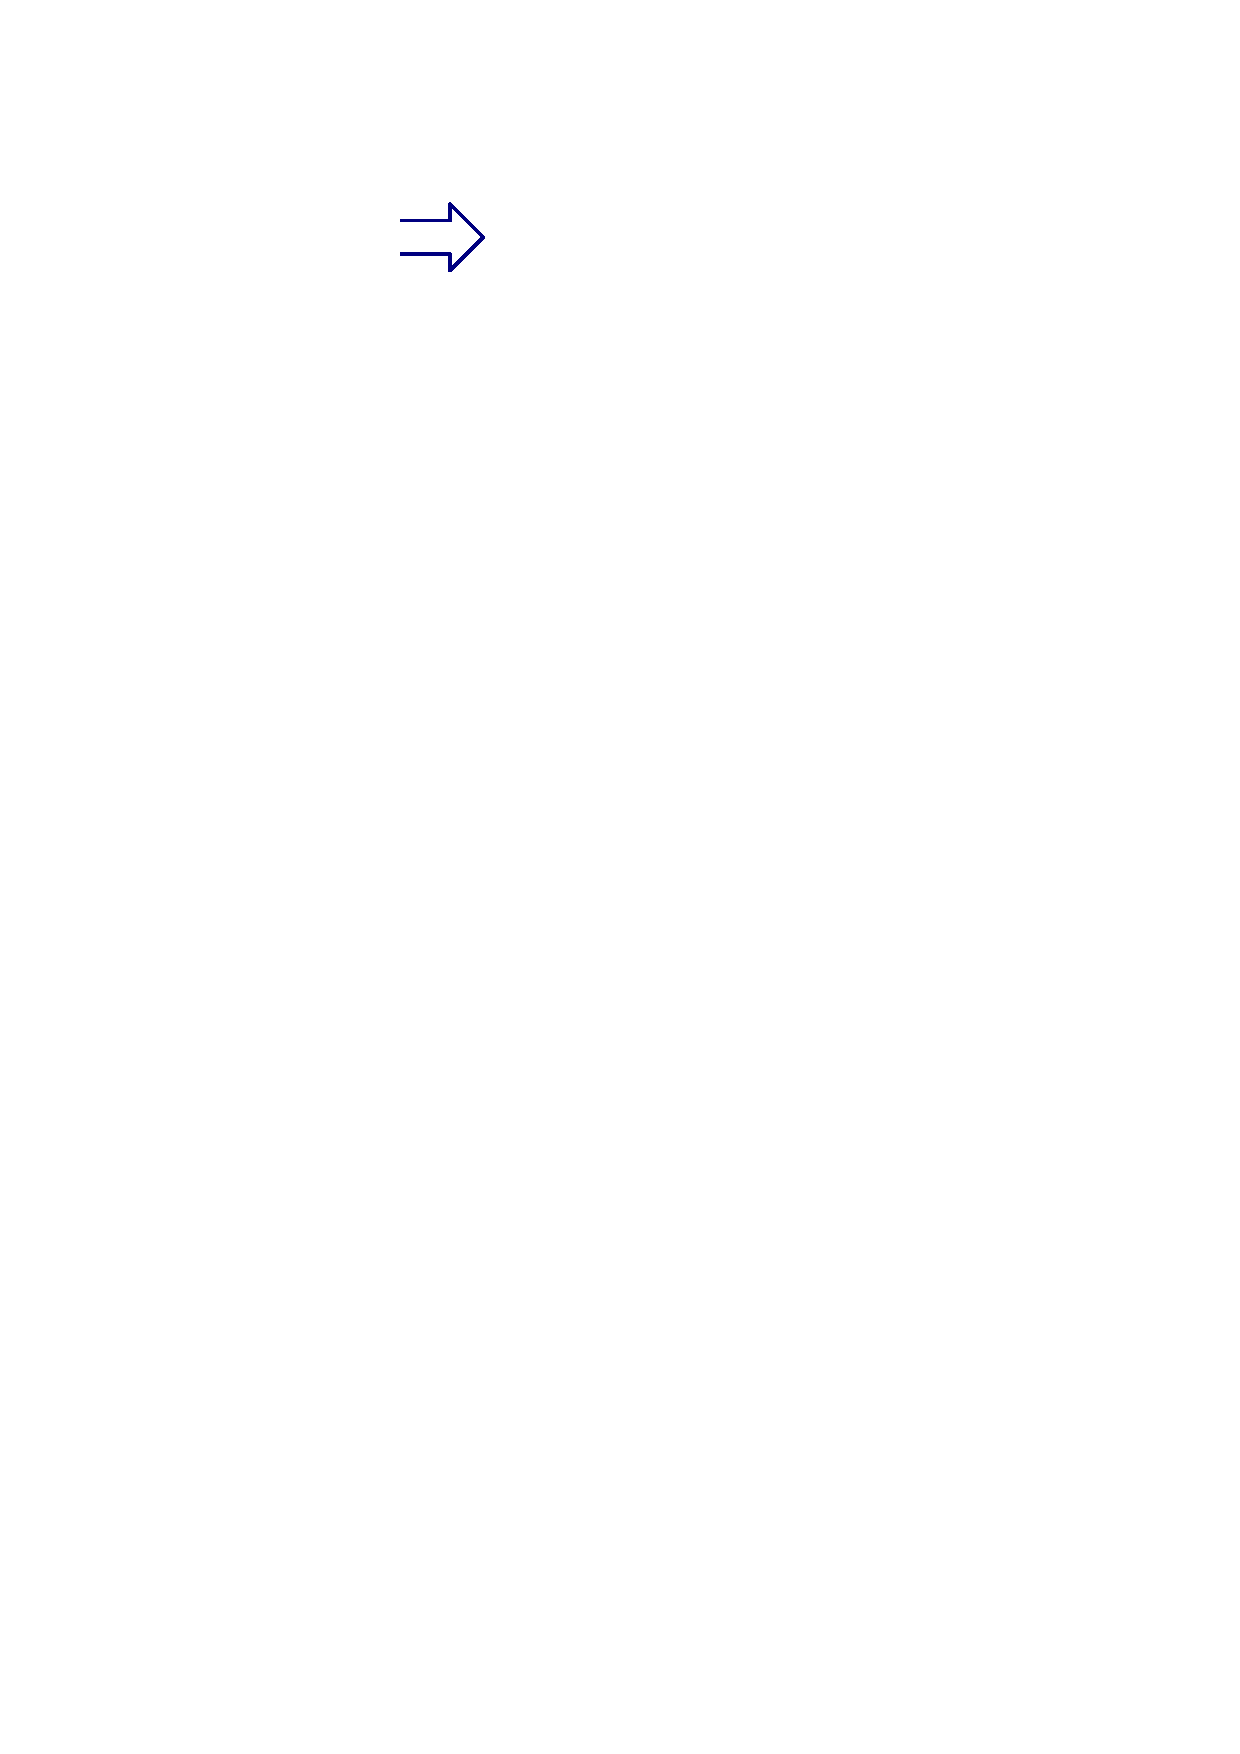
\includegraphics[scale=0.7]{images/arrow.ipe.pdf}
		\end{column}
		\begin{column}{0.16\textwidth}
			\centering
			\scalebox{0.13}{%
				% Scale factor 0.02617801047120419
\definecolor{color54}{RGB}{222,239,234}
\definecolor{color55}{RGB}{255,255,255}
\definecolor{color56}{RGB}{255,255,153}
\definecolor{color57}{RGB}{255,153,153}
\definecolor{color58}{RGB}{0,150,60}
\definecolor{color59}{RGB}{255,0,0}
\definecolor{color60}{RGB}{0,0,0}
% Bounding Box: 573.0, 1806.0
\begin{tikzpicture}
	\node[fill=color54, draw, minimum width=2.4083769633507854cm, minimum height=2.260317128366201cm] (n158) at (4.712041884816754cm ,38.35444278117874cm) {};
	% 1 node layouts
	\node[scale=0.9519276534983341, transform shape] at (4.712041884816754cm ,39.14700915052004cm) {Block  214};
	\node[fill=color54, draw, minimum width=8.638743455497382cm, minimum height=5.672466717465386cm] (n159) at (4.712041884816754cm ,33.34093043941478cm) {};
	% 1 node layouts
	\node[scale=0.9519276534983341, transform shape] at (4.712041884816754cm ,35.83957160330568cm) {Block  175};
	\node[fill=color54, draw, minimum width=2.4083769633507854cm, minimum height=2.260317128366201cm] (n160) at (7.827225130890052cm ,28.327418097650817cm) {};
	% 1 node layouts
	\node[scale=0.9519276534983341, transform shape] at (7.827225130890052cm ,29.119984466992122cm) {Block  215};
	\node[fill=color54, draw, minimum width=6.5706806282722505cm, minimum height=5.672466717465386cm] (n161) at (7.827225130890052cm ,23.313905755886857cm) {};
	% 1 node layouts
	\node[scale=0.9519276534983341, transform shape] at (7.827225130890052cm ,25.812546919777756cm) {Block  176};
	\node[fill=color54, draw, minimum width=2.4083769633507854cm, minimum height=2.260317128366201cm] (n162) at (9.908376963350785cm ,18.300393414122897cm) {};
	% 1 node layouts
	\node[scale=0.9519276534983341, transform shape] at (9.908376963350785cm ,19.092959783464202cm) {Block  216};
	\node[fill=color54, draw, minimum width=6.570680628272251cm, minimum height=5.672466717465386cm] (n163) at (9.908376963350785cm ,13.286881072358936cm) {};
	% 1 node layouts
	\node[scale=0.9519276534983341, transform shape] at (9.908376963350785cm ,15.785522236249834cm) {Block  177};
	\node[fill=color54, draw, minimum width=2.4083769633507854cm, minimum height=2.260317128366201cm] (n164) at (11.989528795811518cm ,8.273368730594974cm) {};
	% 1 node layouts
	\node[scale=0.9519276534983341, transform shape] at (11.989528795811518cm ,9.065935099936281cm) {Block  217};
	\node[fill=color54, draw, minimum width=6.570680628272251cm, minimum height=5.672466717465386cm] (n165) at (11.989528795811518cm ,3.2598563888310137cm) {};
	% 1 node layouts
	\node[scale=0.9519276534983341, transform shape] at (11.989528795811518cm ,5.758497552721912cm) {Block  178};
	\node[fill=color54, draw, minimum width=2.4083769633507854cm, minimum height=2.260317128366201cm] (n166) at (14.070680628272251cm ,-1.753655952932947cm) {};
	% 1 node layouts
	\node[scale=0.9519276534983341, transform shape] at (14.070680628272251cm ,-0.9610895835916409cm) {Block  218};
	\node[fill=color54, draw, minimum width=2.643979057591623cm, minimum height=3.830997756638452cm] (n167) at (14.070680628272251cm ,-5.846433814283441cm) {};
	% 1 node layouts
	\node[scale=0.9519276534983341, transform shape] at (14.070680628272251cm ,-4.268527130806009cm) {Block  77};
	\node[fill=color55, draw, minimum width=1.9109947643979057cm, minimum height=0.7943485419787661cm] (n168) at (7.270942408376963cm ,22.83819745348386cm) {};
	% 1 node layouts
	\node[scale=0.9519276534983341, transform shape] at (7.270942408376963cm ,22.83819745348386cm) {Add Is 172};
	\node[fill=color56, draw, minimum width=2.5916230366492146cm, minimum height=0.7943485419787661cm] (n169) at (6.230366492146597cm ,24.679666414310795cm) {};
	% 1 node layouts
	\node[scale=0.9519276534983341, transform shape] at (6.230366492146597cm ,24.679666414310795cm) {Const 0x1 Is 84};
	\node[fill=color57, draw, minimum width=1.6230366492146597cm, minimum height=0.7943485419787661cm] (n170) at (9.908376963350785cm ,24.679666414310795cm) {};
	% 1 node layouts
	\node[scale=0.9519276534983341, transform shape] at (9.908376963350785cm ,24.679666414310795cm) {Jmp  188};
	\node[fill=color58, draw, minimum width=0.5235602094240838cm, minimum height=0.5235602094240838cm] (n171) at (8.311518324607329cm ,24.679666414310795cm) {};
	\node[fill=color58, draw, minimum width=0.5235602094240838cm, minimum height=0.5235602094240838cm] (n172) at (7.270942408376963cm ,21.132122658934268cm) {};
	\node[fill=color55, draw, minimum width=1.9109947643979057cm, minimum height=0.7943485419787661cm] (n173) at (3.6387434554973823cm ,32.865222137011784cm) {};
	% 1 node layouts
	\node[scale=0.9519276534983341, transform shape] at (3.6387434554973823cm ,32.865222137011784cm) {Add Is 171};
	\node[fill=color56, draw, minimum width=2.5916230366492146cm, minimum height=0.7943485419787661cm] (n174) at (2.081151832460733cm ,34.706691097838714cm) {};
	% 1 node layouts
	\node[scale=0.9519276534983341, transform shape] at (2.081151832460733cm ,34.706691097838714cm) {Const 0x0 Is 72};
	\node[fill=color56, draw, minimum width=2.5916230366492146cm, minimum height=0.7943485419787661cm] (n175) at (5.196335078534031cm ,34.706691097838714cm) {};
	% 1 node layouts
	\node[scale=0.9519276534983341, transform shape] at (5.196335078534031cm ,34.706691097838714cm) {Const 0x1 Is 84};
	\node[fill=color57, draw, minimum width=1.6230366492146597cm, minimum height=0.7943485419787661cm] (n176) at (7.827225130890052cm ,34.706691097838714cm) {};
	% 1 node layouts
	\node[scale=0.9519276534983341, transform shape] at (7.827225130890052cm ,34.706691097838714cm) {Jmp  187};
	\node[fill=color58, draw, minimum width=0.5235602094240838cm, minimum height=0.5235602094240838cm] (n177) at (3.6387434554973823cm ,31.15914734246219cm) {};
	\node[fill=color57, draw, minimum width=1.6230366492146597cm, minimum height=0.7943485419787661cm] (n178) at (14.070680628272251cm ,-2.0939700890586015cm) {};
	% 1 node layouts
	\node[scale=0.9519276534983341, transform shape] at (14.070680628272251cm ,-2.0939700890586015cm) {Jmp  203};
	\node[fill=color57, draw, minimum width=1.8586387434554974cm, minimum height=0.7943485419787661cm] (n179) at (14.070680628272251cm ,-6.972088264545221cm) {};
	% 1 node layouts
	\node[scale=0.9519276534983341, transform shape] at (14.070680628272251cm ,-6.972088264545221cm) {Return  87};
	\node[fill=color58, draw, minimum width=0.5235602094240838cm, minimum height=0.5235602094240838cm] (n180) at (13.547120418848168cm ,-5.266013469995628cm) {};
	\node[fill=color57, draw, minimum width=1.6230366492146597cm, minimum height=0.7943485419787661cm] (n181) at (11.989528795811518cm ,7.93305459446932cm) {};
	% 1 node layouts
	\node[scale=0.9519276534983341, transform shape] at (11.989528795811518cm ,7.93305459446932cm) {Jmp  200};
	\node[fill=color57, draw, minimum width=1.6230366492146597cm, minimum height=0.7943485419787661cm] (n182) at (4.712041884816754cm ,38.014128645053084cm) {};
	% 1 node layouts
	\node[scale=0.9519276534983341, transform shape] at (4.712041884816754cm ,38.014128645053084cm) {Jmp  194};
	\node[fill=color57, draw, minimum width=1.6230366492146597cm, minimum height=0.7943485419787661cm] (n183) at (9.908376963350785cm ,17.96007927799724cm) {};
	% 1 node layouts
	\node[scale=0.9519276534983341, transform shape] at (9.908376963350785cm ,17.96007927799724cm) {Jmp  198};
	\node[fill=color57, draw, minimum width=1.6230366492146597cm, minimum height=0.7943485419787661cm] (n184) at (7.827225130890052cm ,27.987103961525165cm) {};
	% 1 node layouts
	\node[scale=0.9519276534983341, transform shape] at (7.827225130890052cm ,27.987103961525165cm) {Jmp  196};
	\node[fill=color55, draw, minimum width=1.9109947643979057cm, minimum height=0.7943485419787661cm] (n185) at (11.43324607329843cm ,2.784148086428018cm) {};
	% 1 node layouts
	\node[scale=0.9519276534983341, transform shape] at (11.43324607329843cm ,2.784148086428018cm) {Add Is 174};
	\node[fill=color56, draw, minimum width=2.5916230366492146cm, minimum height=0.7943485419787661cm] (n186) at (10.392670157068062cm ,4.625617047254952cm) {};
	% 1 node layouts
	\node[scale=0.9519276534983341, transform shape] at (10.392670157068062cm ,4.625617047254952cm) {Const 0x1 Is 84};
	\node[fill=color57, draw, minimum width=1.6230366492146597cm, minimum height=0.7943485419787661cm] (n187) at (14.070680628272251cm ,4.625617047254952cm) {};
	% 1 node layouts
	\node[scale=0.9519276534983341, transform shape] at (14.070680628272251cm ,4.625617047254952cm) {Jmp  190};
	\node[fill=color58, draw, minimum width=0.5235602094240838cm, minimum height=0.5235602094240838cm] (n188) at (12.473821989528796cm ,4.625617047254952cm) {};
	\node[fill=color58, draw, minimum width=0.5235602094240838cm, minimum height=0.5235602094240838cm] (n189) at (11.43324607329843cm ,1.0780732918784257cm) {};
	\node[fill=color55, draw, minimum width=1.9109947643979057cm, minimum height=0.7943485419787661cm] (n190) at (9.352094240837696cm ,12.81117276995594cm) {};
	% 1 node layouts
	\node[scale=0.9519276534983341, transform shape] at (9.352094240837696cm ,12.81117276995594cm) {Add Is 173};
	\node[fill=color56, draw, minimum width=2.5916230366492146cm, minimum height=0.7943485419787661cm] (n191) at (8.311518324607329cm ,14.652641730782873cm) {};
	% 1 node layouts
	\node[scale=0.9519276534983341, transform shape] at (8.311518324607329cm ,14.652641730782873cm) {Const 0x1 Is 84};
	\node[fill=color57, draw, minimum width=1.6230366492146597cm, minimum height=0.7943485419787661cm] (n192) at (11.989528795811518cm ,14.652641730782873cm) {};
	% 1 node layouts
	\node[scale=0.9519276534983341, transform shape] at (11.989528795811518cm ,14.652641730782873cm) {Jmp  189};
	\node[fill=color58, draw, minimum width=0.5235602094240838cm, minimum height=0.5235602094240838cm] (n193) at (10.392670157068062cm ,14.652641730782873cm) {};
	\node[fill=color58, draw, minimum width=0.5235602094240838cm, minimum height=0.5235602094240838cm] (n194) at (9.352094240837696cm ,11.105097975406347cm) {};
	\draw[color=color59, -latex] (4.712041884816754cm ,36.17716379814747cm) -- (4.712041884816754cm ,37.6169543740637cm);
	\node[] at (4.908376963350786cm ,36.70850037280177cm) {
		\scalebox{0.9519276534983341}{0}
	};
	\draw[color=color59, -latex] (7.827225130890052cm ,29.45757666183392cm) -- (7.827225130890052cm ,34.30951682684933cm);
	\node[] at (8.023560209424083cm ,29.988913236488223cm) {
		\scalebox{0.9519276534983341}{0}
	};
	\draw[color=color59, -latex] (7.827225130890052cm ,26.15013911461955cm) -- (7.827225130890052cm ,27.58992969053578cm);
	\node[] at (8.023560209424083cm ,26.681475689273853cm) {
		\scalebox{0.9519276534983341}{0}
	};
	\draw[color=color59, -latex] (9.908376963350785cm ,19.430551978305996cm) -- (9.908376963350785cm ,24.282492143321413cm);
	\node[] at (10.104712041884817cm ,19.9618885529603cm) {
		\scalebox{0.9519276534983341}{0}
	};
	\draw[color=color59, -latex] (9.908376963350785cm ,16.12311443109163cm) -- (9.908376963350785cm ,17.56290500700786cm);
	\node[] at (10.104712041884817cm ,16.654451005745933cm) {
		\scalebox{0.9519276534983341}{0}
	};
	\draw[color=color59, -latex] (11.989528795811518cm ,9.403527294778074cm) -- (11.989528795811518cm ,14.25546745979349cm);
	\node[] at (12.18586387434555cm ,9.934863869432379cm) {
		\scalebox{0.9519276534983341}{0}
	};
	\draw[color=color59, -latex] (11.989528795811518cm ,6.096089747563707cm) -- (11.989528795811518cm ,7.535880323479937cm);
	\node[] at (12.18586387434555cm ,6.627426322218011cm) {
		\scalebox{0.9519276534983341}{0}
	};
	\draw[color=color59, -latex] (14.070680628272251cm ,-0.6234973887498466cm) -- (14.070680628272251cm ,4.2284427762655685cm);
	\node[] at (14.267015706806284cm ,-0.09216081409554207cm) {
		\scalebox{0.9519276534983341}{0}
	};
	\draw[color=color59, -latex] (14.070680628272251cm ,-3.9309349359642147cm) -- (14.070680628272251cm ,-2.4911443600479846cm);
	\node[] at (14.267015706806284cm ,-3.39959836130991cm) {
		\scalebox{0.9519276534983341}{0}
	};
	\draw[color=color60, -latex] (6.793193717277487cm ,23.235371724473243cm) -- (6.793193717277487cm ,23.758931933897326cm) -- (6.230366492146597cm ,23.758931933897326cm) -- (6.230366492146597cm ,24.282492143321413cm);
	\node[] at (6.989528795811518cm ,23.616589001960154cm) {
		\scalebox{0.9519276534983341}{1}
	};
	\draw[color=color60, -latex] (7.7486910994764395cm ,23.235371724473243cm) -- (7.7486910994764395cm ,23.758931933897326cm) -- (8.311518324607329cm ,23.758931933897326cm) -- (8.311518324607329cm ,24.417886309598753cm);
	\node[] at (7.945026178010471cm ,23.616589001960154cm) {
		\scalebox{0.9519276534983341}{0}
	};
	\draw[color=color60, -latex] (7.270942408376963cm ,21.39390276364631cm) -- (7.270942408376963cm ,22.44102318249448cm);
	\node[] at (7.467277486910994cm ,21.917462973070393cm) {
		\scalebox{0.9519276534983341}{0}
	};
	\draw[color=color60, -latex] (3.160994764397906cm ,33.262396408001166cm) -- (3.160994764397906cm ,33.78595661742525cm) -- (2.081151832460733cm ,33.78595661742525cm) -- (2.081151832460733cm ,34.30951682684933cm);
	\node[] at (3.357329842931937cm ,33.64361368548808cm) {
		\scalebox{0.9519276534983341}{0}
	};
	\draw[color=color60, -latex] (4.116492146596858cm ,33.262396408001166cm) -- (4.116492146596858cm ,33.78595661742525cm) -- (5.196335078534031cm ,33.78595661742525cm) -- (5.196335078534031cm ,34.30951682684933cm);
	\node[] at (4.31282722513089cm ,33.64361368548808cm) {
		\scalebox{0.9519276534983341}{1}
	};
	\draw[color=color60, -latex] (3.6387434554973823cm ,31.420927447174233cm) -- (3.6387434554973823cm ,32.4680478660224cm);
	\node[] at (3.8350785340314135cm ,31.944487656598316cm) {
		\scalebox{0.9519276534983341}{0}
	};
	\draw[color=color60, -latex] (13.606020942408376cm ,-6.574913993555838cm) -- (13.606020942408376cm ,-6.051353784131754cm) -- (13.547120418848168cm ,-6.051353784131754cm) -- (13.547120418848168cm ,-5.527793574707671cm);
	\node[] at (13.802356020942408cm ,-6.193696716068927cm) {
		\scalebox{0.9519276534983341}{1}
	};
	\draw[color=color60, -latex] (10.955497382198953cm ,3.181322357417401cm) -- (10.955497382198953cm ,3.704882566841485cm) -- (10.392670157068062cm ,3.704882566841485cm) -- (10.392670157068062cm ,4.2284427762655685cm);
	\node[] at (11.151832460732985cm ,3.5625396349043124cm) {
		\scalebox{0.9519276534983341}{1}
	};
	\draw[color=color60, -latex] (11.910994764397905cm ,3.181322357417401cm) -- (11.910994764397905cm ,3.704882566841485cm) -- (12.473821989528796cm ,3.704882566841485cm) -- (12.473821989528796cm ,4.3638369425429095cm);
	\node[] at (12.107329842931938cm ,3.5625396349043124cm) {
		\scalebox{0.9519276534983341}{0}
	};
	\draw[color=color60, -latex] (11.43324607329843cm ,1.3398533965904675cm) -- (11.43324607329843cm ,2.386973815438635cm);
	\node[] at (11.629581151832461cm ,1.8634136060145512cm) {
		\scalebox{0.9519276534983341}{1}
	};
	\draw[color=color60, -latex] (8.87434554973822cm ,13.208347040945323cm) -- (8.87434554973822cm ,13.731907250369407cm) -- (8.311518324607329cm ,13.731907250369407cm) -- (8.311518324607329cm ,14.25546745979349cm);
	\node[] at (9.070680628272251cm ,13.589564318432233cm) {
		\scalebox{0.9519276534983341}{1}
	};
	\draw[color=color60, -latex] (9.829842931937172cm ,13.208347040945323cm) -- (9.829842931937172cm ,13.731907250369407cm) -- (10.392670157068062cm ,13.731907250369407cm) -- (10.392670157068062cm ,14.390861626070832cm);
	\node[] at (10.026178010471204cm ,13.589564318432233cm) {
		\scalebox{0.9519276534983341}{0}
	};
	\draw[color=color60, -latex] (9.352094240837696cm ,11.366878080118388cm) -- (9.352094240837696cm ,12.413998498966556cm);
	\node[] at (9.548429319371728cm ,11.890438289542473cm) {
		\scalebox{0.9519276534983341}{0}
	};
\end{tikzpicture}

			}
		\end{column}
	\end{columns}
\end{frame}






\section{Backend}

\begin{frame}
	\frametitle{Instruction Selection}
	\begin{columns}
		\begin{column}{0.55\textwidth}
			\begin{itemize}
				\item Uses simplified bottom-up pattern matching
				\item Does not resolve $\phi$-Instructions
			\end{itemize}

			\vspace{1em}

			\begin{contentblock}{Phase 1: Match Nodes}
				\begin{itemize}
					\item Match each node against (multiple) patterns
					\item Accept first matching pattern (no cost function)
				\end{itemize}
			\end{contentblock}

			\begin{contentblock}{Phase 2: Collect Instructions}
				\begin{itemize}
					\item Walk matches in topological order
					\item Ignore unnecessary predecessors
					\item Discard memory dependencies ($\rightarrow$ no reordering)
				\end{itemize}
			\end{contentblock}
		\end{column}
		\begin{column}{0.44\textwidth}
		 	\centering 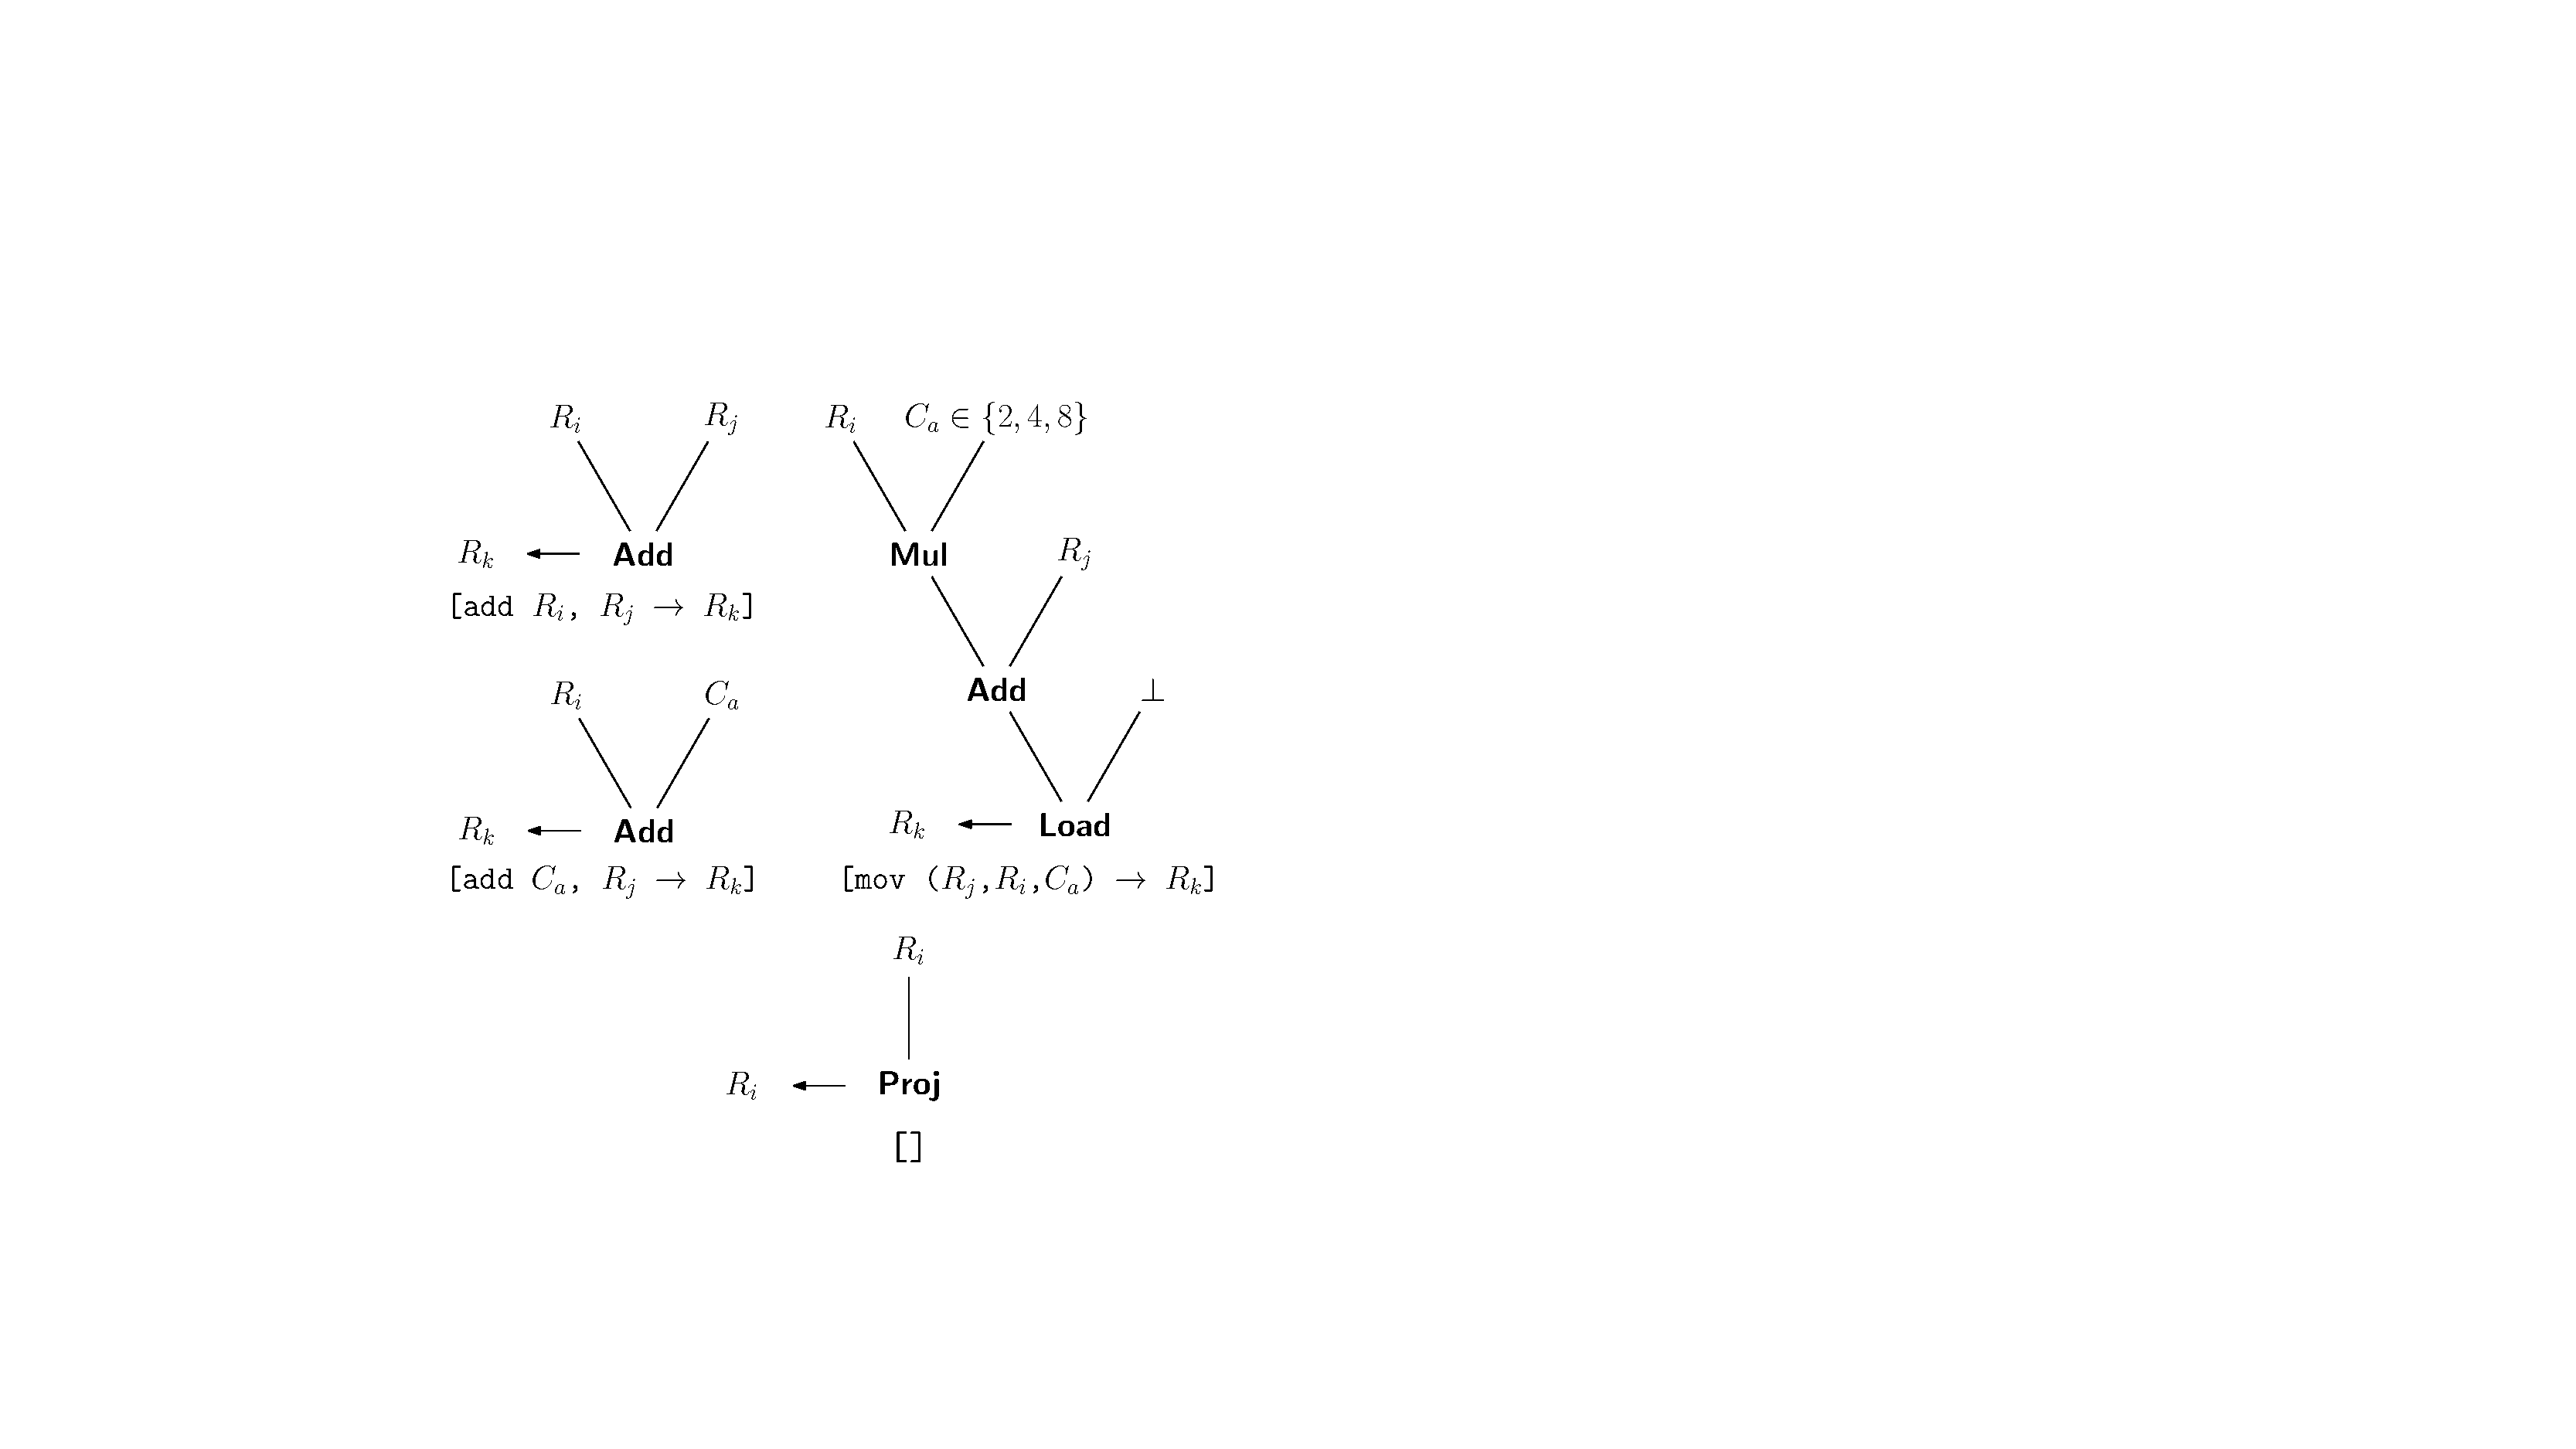
\includegraphics[scale=0.4]{images/pattern.ipe.pdf}
		\end{column}
	\end{columns}

\end{frame}

\begin{frame}
    \frametitle{Register Allocation - Techniques}

    \begin{itemize}
    	\item Blockwise
        \item Linear Scan
        \item Graph Coloring
    \end{itemize}

\end{frame}

\begin{frame}
\frametitle{Register Allocator - Overview}

\centering 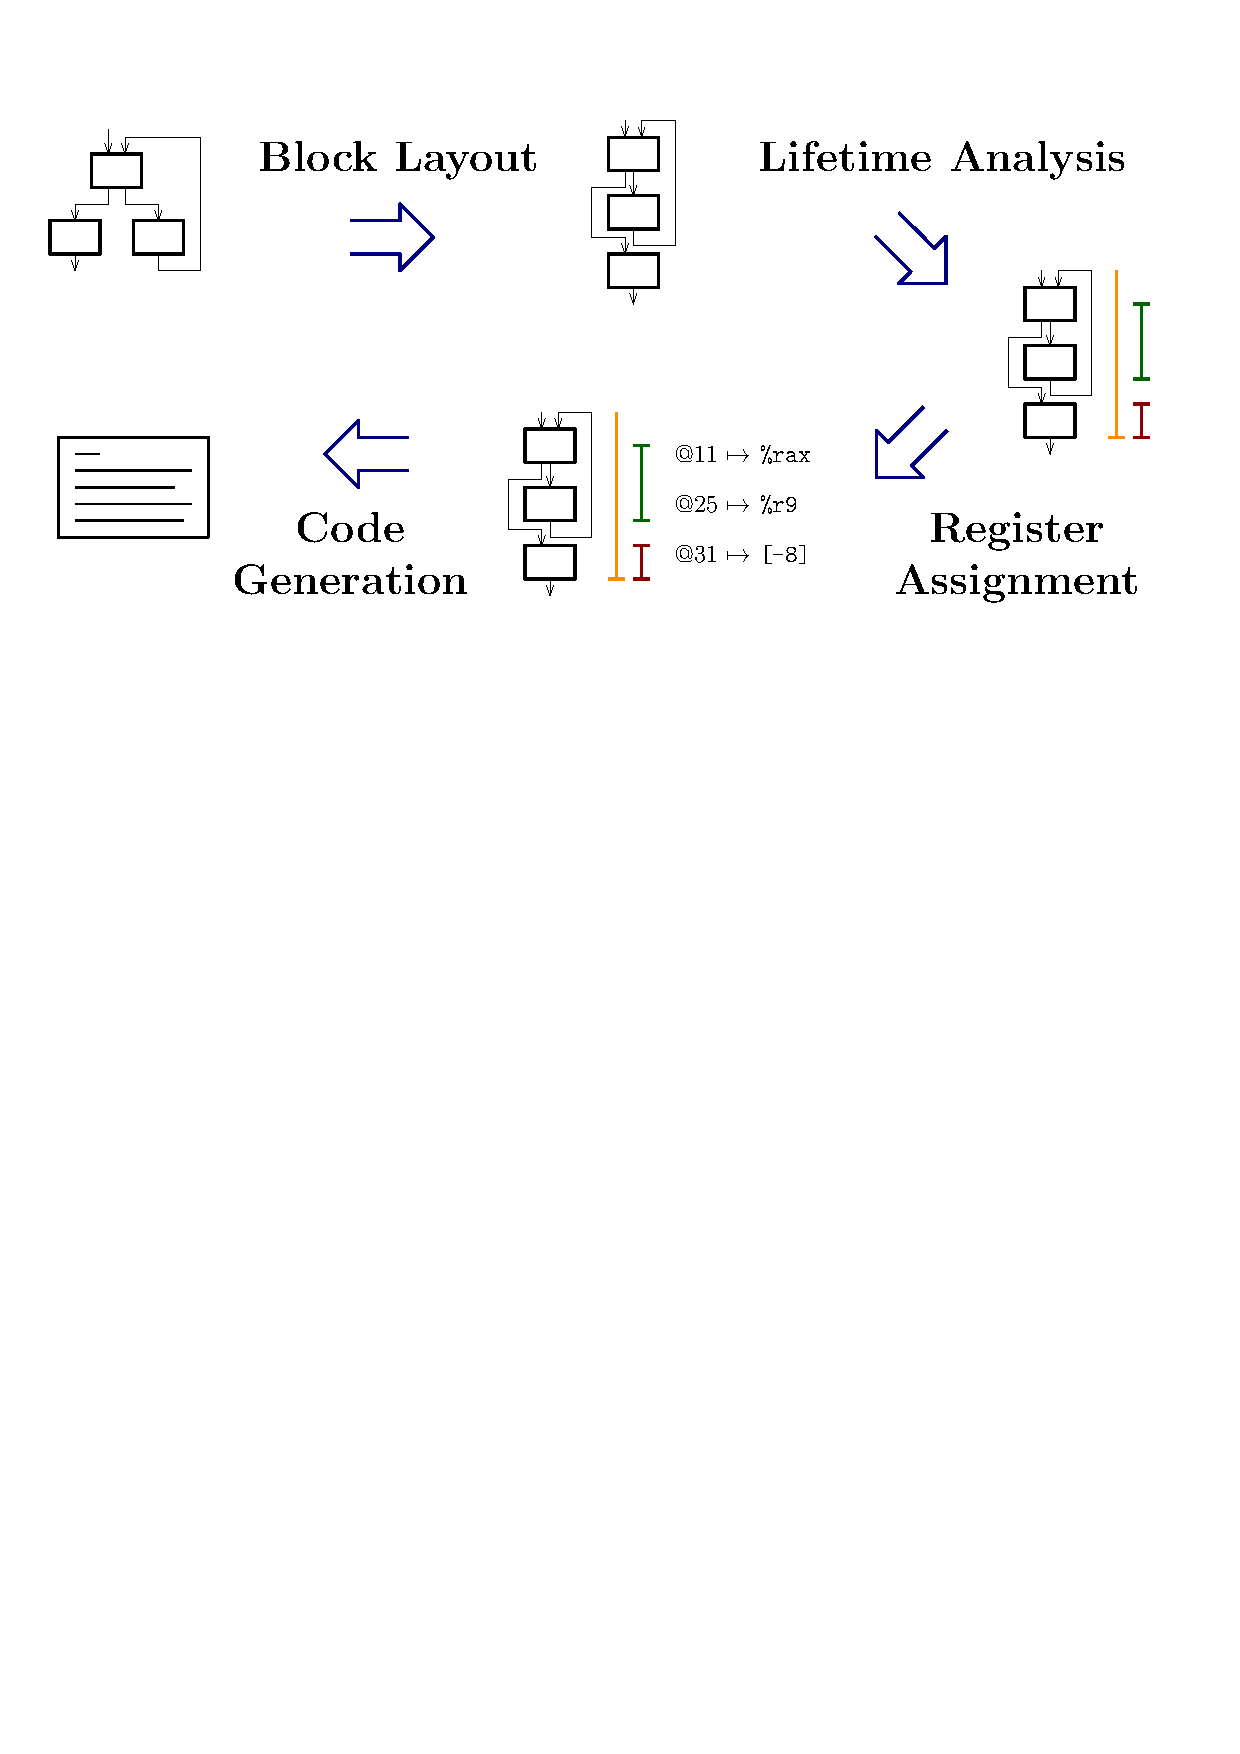
\includegraphics[scale=0.7]{images/overview.pdf}

\end{frame}

\begin{frame}
\frametitle{Register Allocator - Block Layout}

	\begin{columns}
		\begin{column}{0.65\textwidth}
			\begin{itemize}
				\item \textbf{Input:} unordered blocks (intermediate language)
				\item Calculate reverse postfix order
				\item Additionally: loop analysis
					\begin{itemize}
						\item Mapping between blocks and loops
						\item Try to find consecutive block layout for each loop\\ (minimizes lifetime of registers within loop)
					\end{itemize}
				\item \textbf{Output:} linear block ordering, annotated with loop depth
			\end{itemize}
		\end{column}
	
		 \begin{column}{0.35\textwidth}
		 	\centering 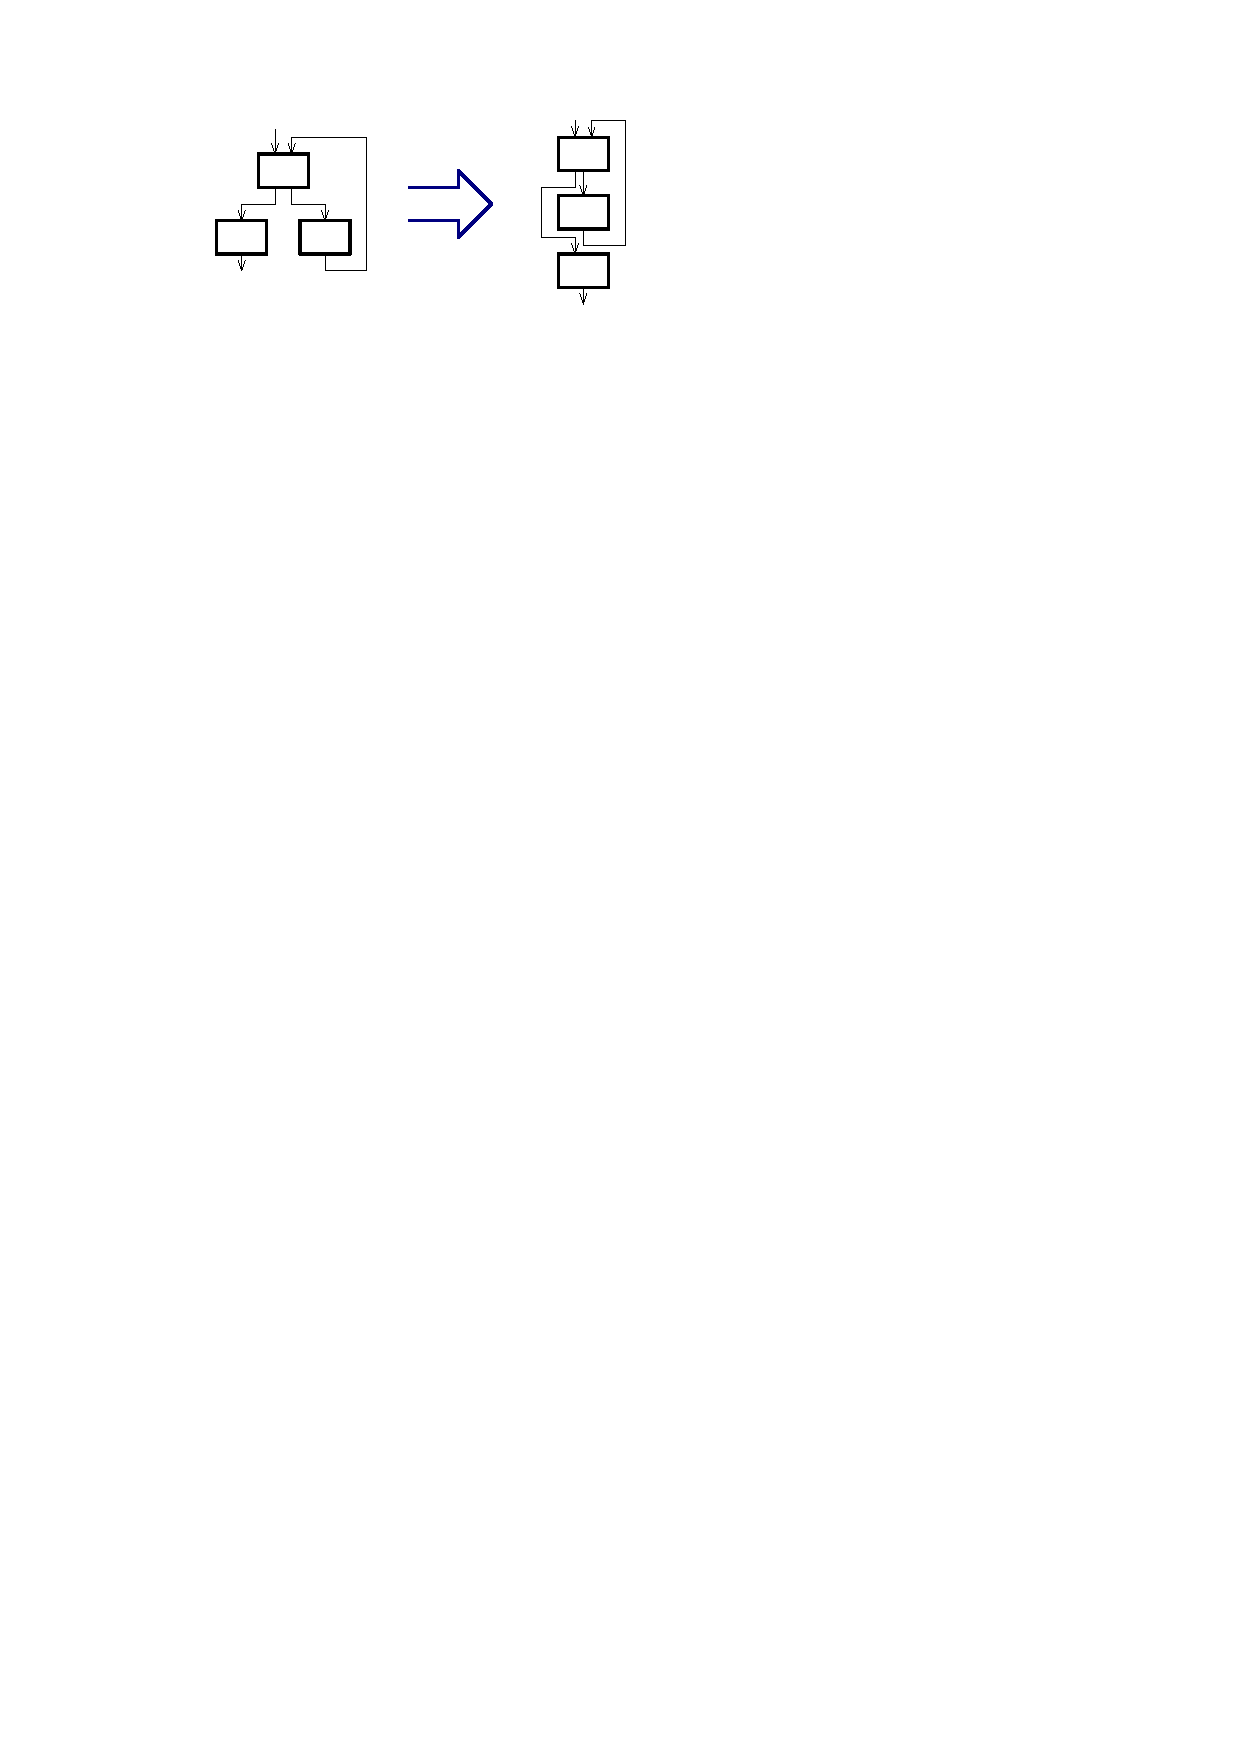
\includegraphics[scale=0.7]{images/block_layout.pdf}
		 \end{column}
	\end{columns}
\end{frame}

\begin{frame}
\frametitle{Register Allocator - Lifetime Analysis}

\begin{columns}
	\begin{column}{0.65\textwidth}
		\begin{itemize}
			\item \textbf{Input:} linearized blocks
			\item Calculate lifetime intervals for each virtual register 
			\begin{itemize}
				\item Definition and last usage
				\item Differentiate input and output (allows reusing registers)
				\item Beware loops: lifetime extension required!
			\end{itemize}
			\item Collect other useful stats for each virtual register
			\begin{itemize}
				\item Loop depth
				\item \texttt{div}, \texttt{mod} and \texttt{call}
			\end{itemize}
			\item \textbf{Output:} register lifetimes and additional stats
		\end{itemize}
	\end{column}
	
	\begin{column}{0.35\textwidth}
		\centering 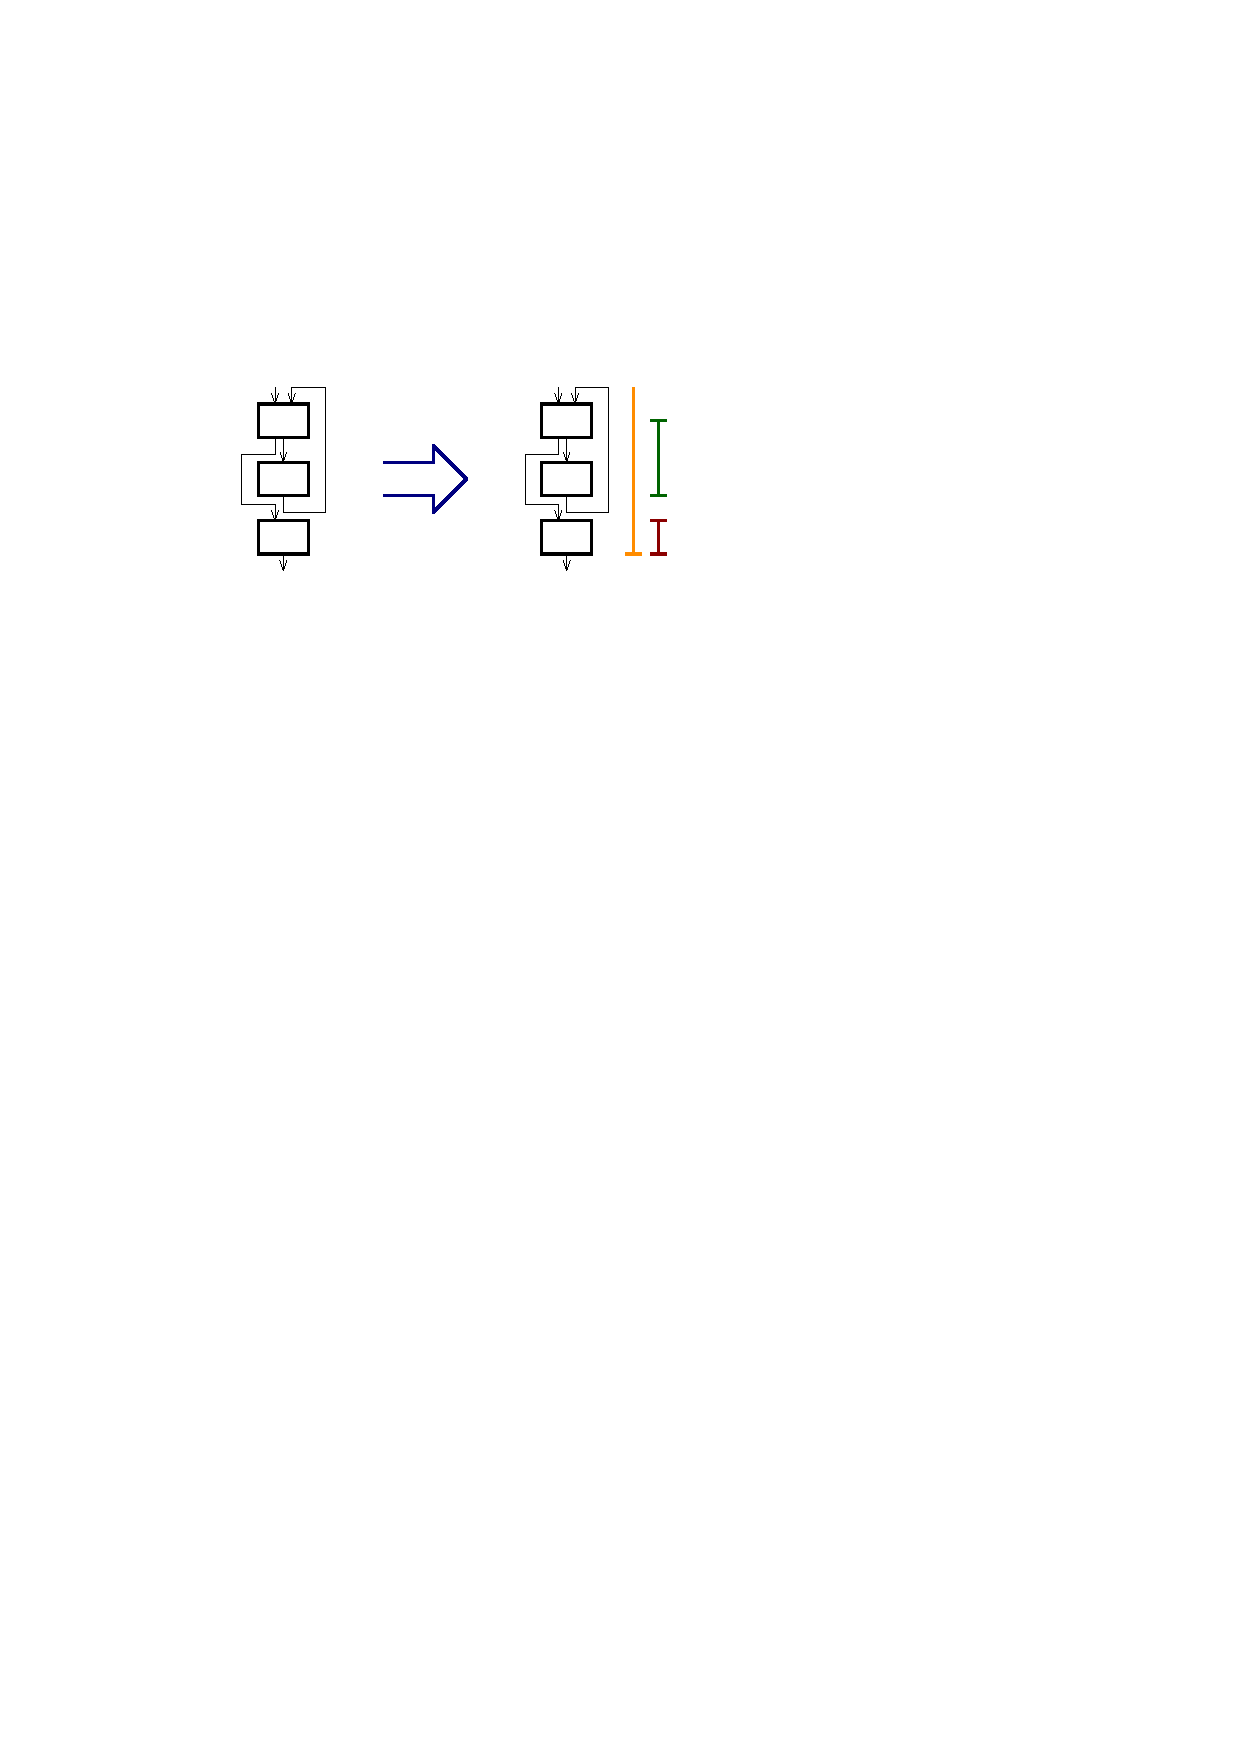
\includegraphics[scale=0.7]{images/lifetimes.pdf}
	\end{column}
\end{columns}
\end{frame}

\begin{frame}
\frametitle{Register Allocator - Register Assignment}

\begin{columns}
	\begin{column}{0.7\textwidth}
		\begin{itemize}
			\item \textbf{Input:} linearized blocks and lifetimes
			\item Assign virtual registers to hardware register or stack slot
			\item Linear scan over blocks, select best assignment greedily
			\item Spill decision based on loop depth and lifetime 
			\begin{itemize}
				\item Always spill for entire lifetime
			\end{itemize}
			\item Considerations when assigning a register:
			\begin{itemize}
				\item Reuse input register if possible
				\item Reduce and/or eliminate moves
				\item Callee-saved register in case of interfering calls
				\item According register for function arguments and return value
			\end{itemize}
			\item \textbf{Output:} register assignment
		\end{itemize}
	\end{column}
	
	\begin{column}{0.3\textwidth}
		\centering 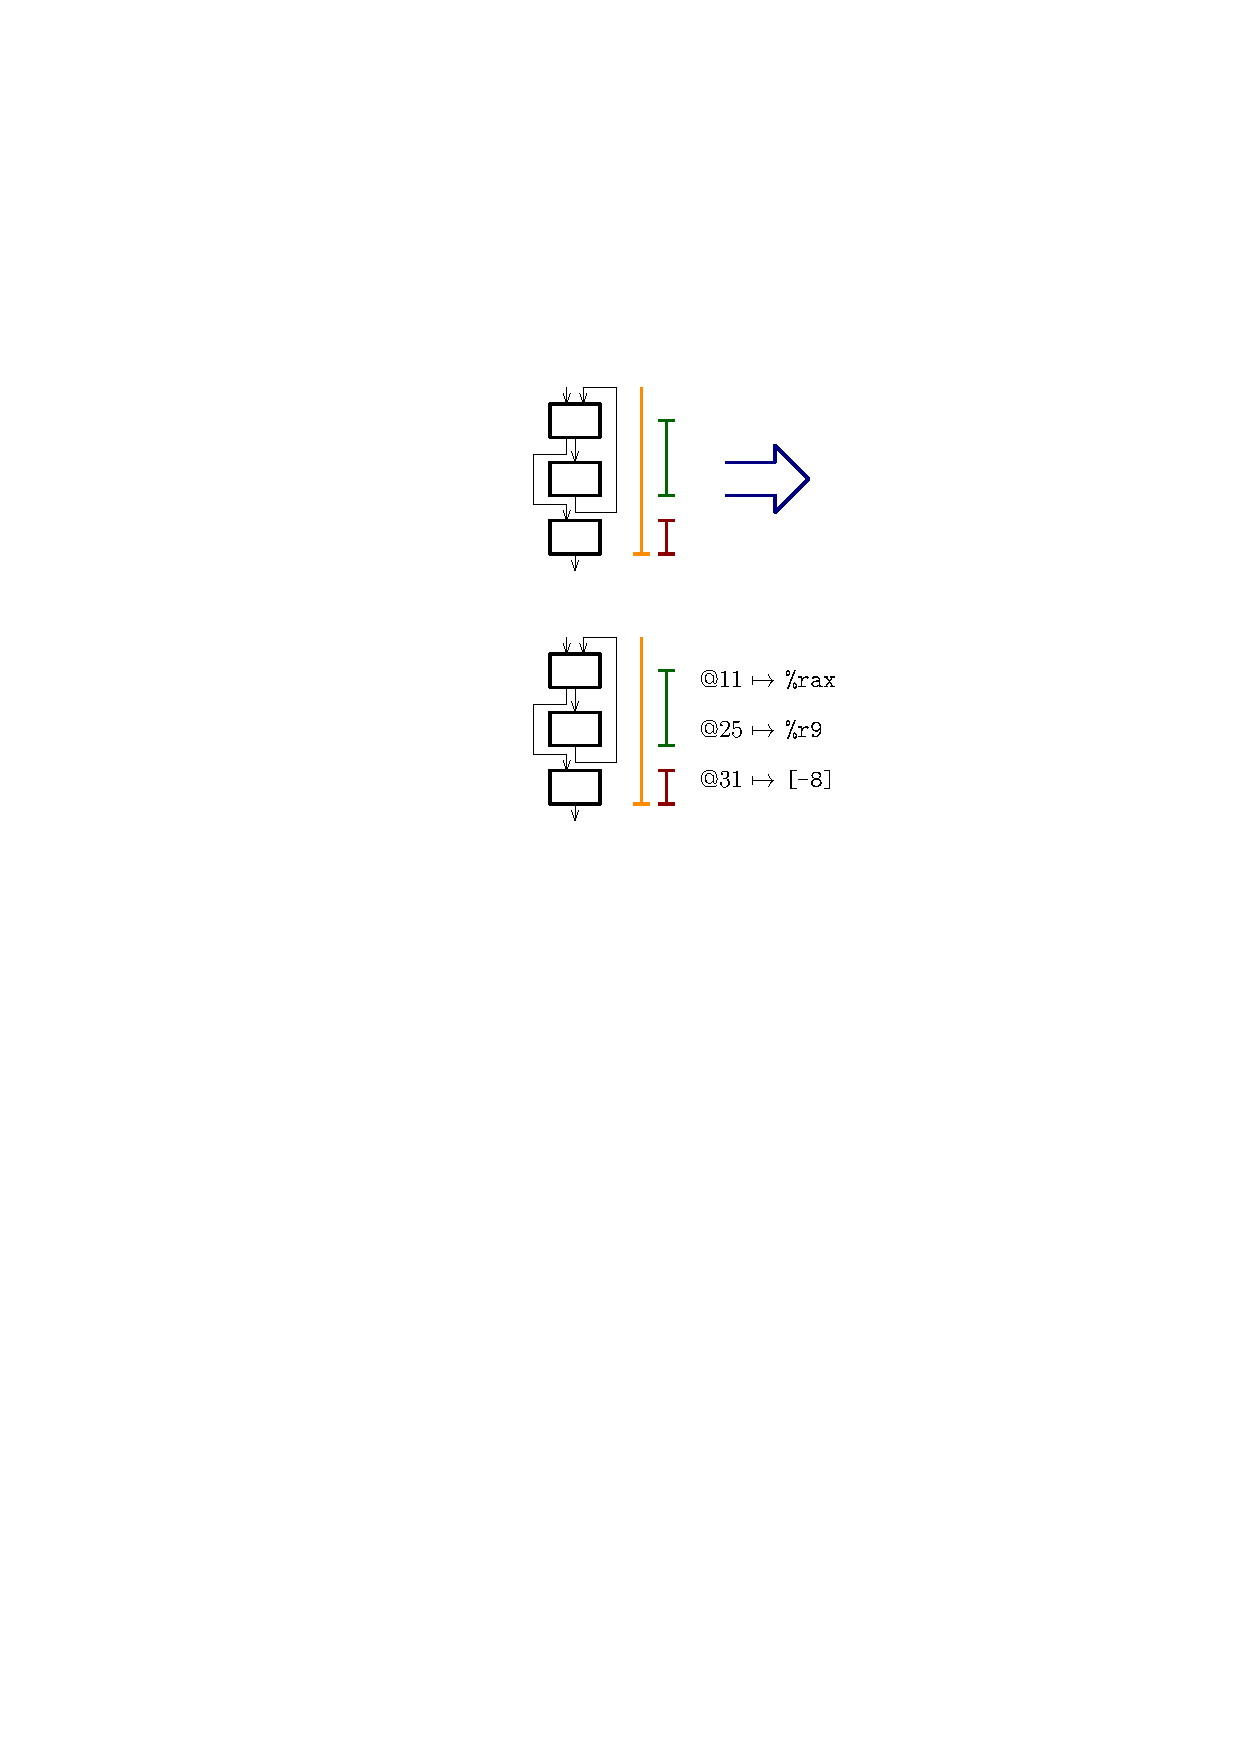
\includegraphics[scale=0.7]{images/allocation.pdf}
	\end{column}
\end{columns}
\end{frame}

\begin{frame}
\frametitle{Register Allocator - Code Generation}

\begin{columns}
	\begin{column}{0.7\textwidth}
		\begin{itemize}
			\item \textbf{Input:} everything from above
			\item Verify assignment and generate the actual assembly
			\begin{itemize}
				\item Replace virtual registers
				\item Allocate temporary registers where needed
				\item Generate moves, spills and calling code
			\end{itemize}
			\item Function prolog and epilog (needs register usage)
			\item \textbf{Output:} assembly
		\end{itemize}
	
		\vspace{10pt}
		\begin{itemize}
			\item Calling convention: \texttt{x86-64} System V
			\begin{itemize}
				\item First six arguments in registers
				\item Efficient implementation via register permutation
			\end{itemize}
		\end{itemize}
	\end{column}
	
	\begin{column}{0.3\textwidth}
		\centering 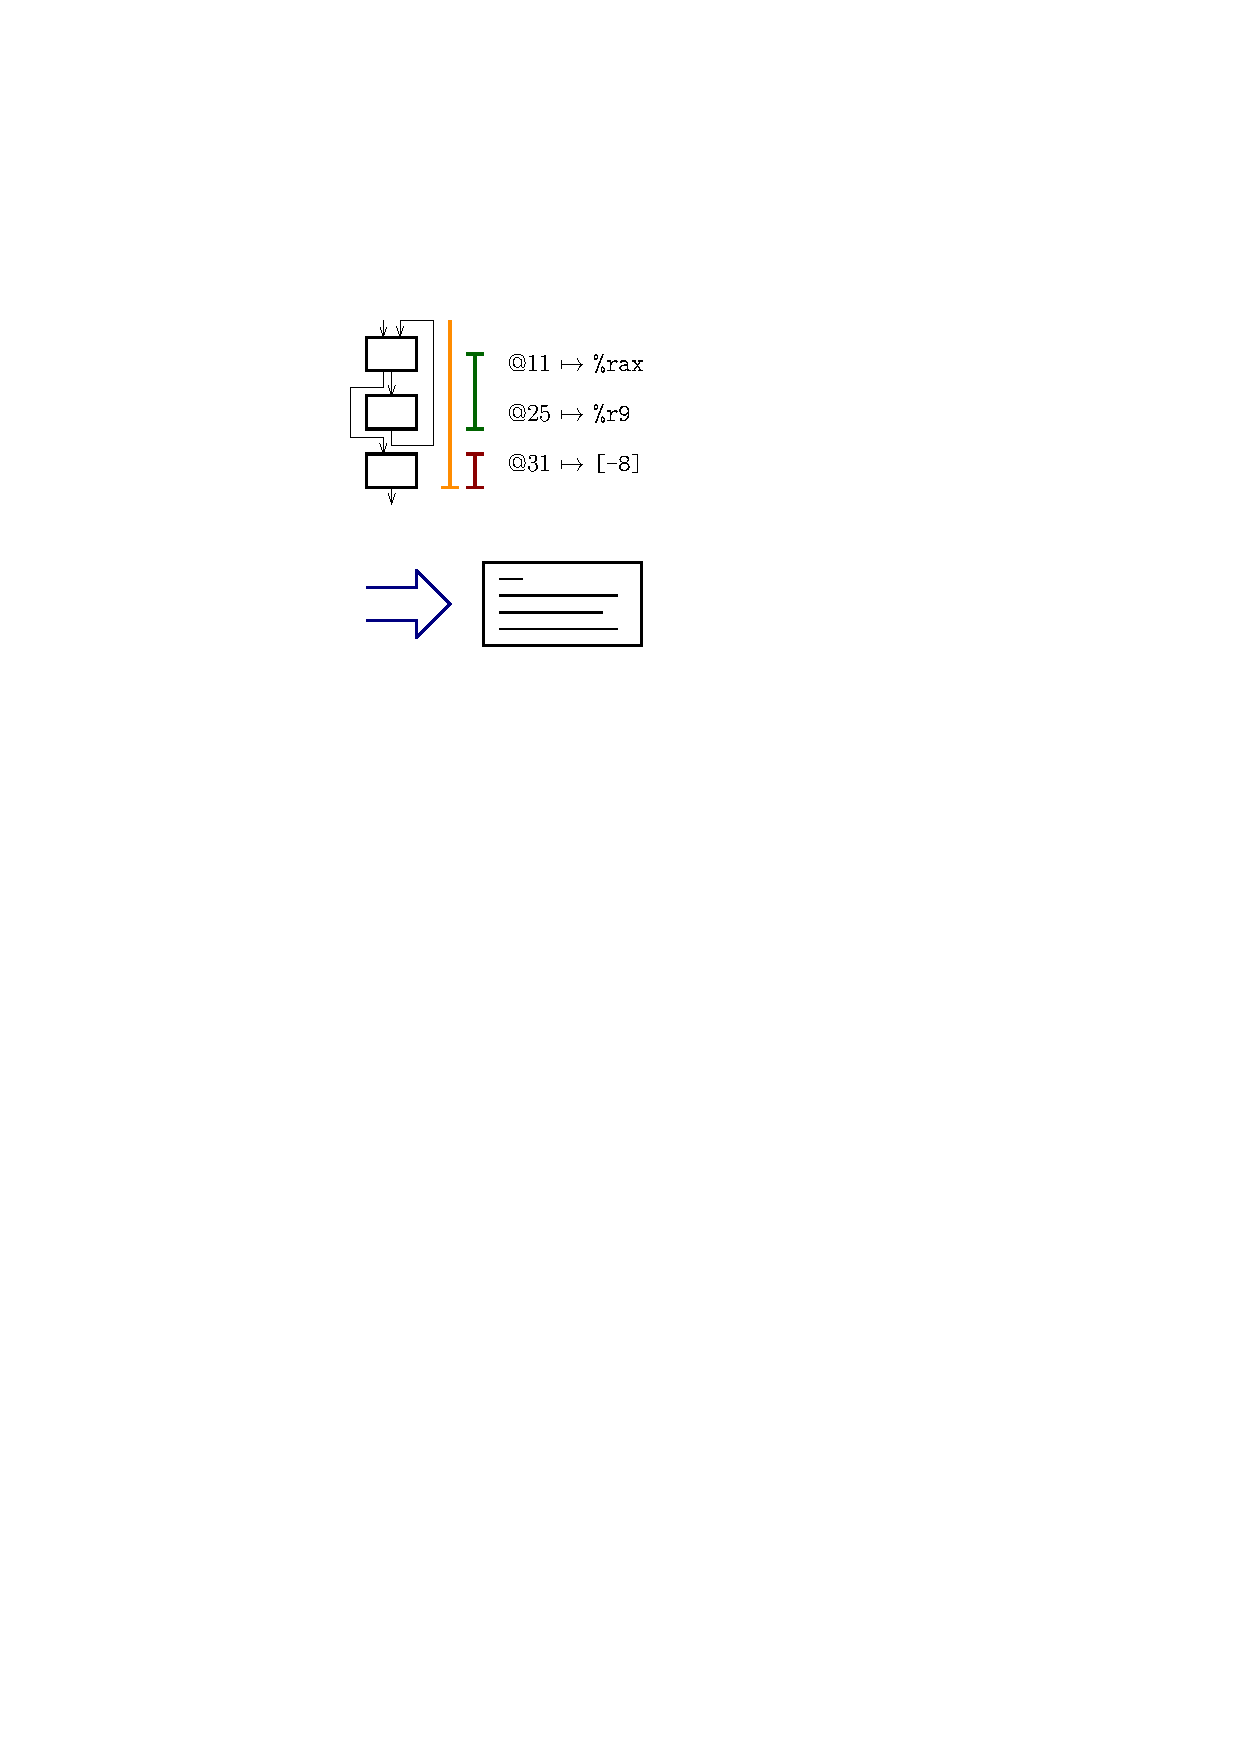
\includegraphics[scale=0.7]{images/code_generation.pdf}
	\end{column}
\end{columns}
\end{frame}

\begin{frame}
    \frametitle{Peephole Optimizations}

    \begin{itemize}
        \item fixed-size (per optimization) window of instructions
        \vspace{1em}
        \item Jump Inversion
    \end{itemize}

\end{frame}

\begin{frame}
    \frametitle{Assembly Output}

    \begin{itemize}
        \item ELF file format
        \item function prologs / epilogs
        \item link runtime library (written in C)
        \item passed to gcc
    \end{itemize}

\end{frame}

\begin{frame}
	\frametitle{Statistics}

	\begin{itemize}
		\item Duration: 16 weeks
		\item Pull requests: 143
		\item LOC: 15'093
		\begin{itemize}
			\item Frontend: 3'812
			\item Middle-End: 5'380
			\item Backend: 5'039
		\end{itemize}
	\end{itemize}

	% graph w/ commits over time

\end{frame}


\begin{frame}
\end{frame}

\appendix
\beginbackup

\backupend

\end{document}
